\chapter{Linear algebra, reprise}
\section{Tensor products and the Tor functors}
In the rest of the chapter we will work in the category $R$-$\mathsf{Mod}$ of modules over a \textit{commutative} ring $R$.
\subsection{Bilinear maps and the definition of tensor product}
If $M$ and $N$ are $R$-modules, $M\oplus N$ serves as both the product and coproduct of $M$ and $N$: a situation in which a limit coincides with a colimit. As a set, $M\oplus N$ is just $M\times N$; the $R$-module structure on $M\oplus N$ is defined by componentwise addition and multiplication by scalars. An $R$-module homomorphism
\[M\oplus N\to P\]
is determined by $R$-module homomorphisms $M\to P$ and $N\to P$ (this is what makes $M\oplus N$ into a coproduct).\par
But there is another way to map $M\times N$ to an $R$-module $P$, compatibly with the $R$-module structures.
\begin{definition}
Let $M,N,P$ be $R$-modules. A function $\varphi:M\times N\to P$ is \textbf{$R$-bilinear} if
\begin{itemize}
\item $\forall m\in M$, the function $n\to\varphi(m,n)$ is an $R$-module homomorphism $N\to P$.
\item $\forall n\in N$, the function $m\to\varphi(m,n)$ is an $R$-module homomorphism $M\to P$.
\end{itemize}
\end{definition}
Thus, if $\varphi:M\times N\to P$ is $R$-bilinear, then $\forall m\in M$, $\forall n_1,n_2\in N$, $\forall r_1,r_2\in R$,
\[\varphi(m,r_1n_1+r_2n_2)=r_1\varphi(m,n_1)+r_2(m,n_2)\]
and similarly for $\varphi(\cdot,n)$.\par
What we need is a new $R$-module $M\otimes_{R}N$, with an $R$-bilinear map
\[\otimes:M\times N\to M\otimes_{R}N\]
such that every $R$-bilinear map $M\times N\to P$ factors uniquely through this new module $M\otimes_{R}N$,
\[\begin{tikzcd}
M\times N\ar[d,swap,"\otimes"]\ar[r,"\varphi"]&P\\
M\otimes_{R}N\ar[ru,swap,"\exists !\varphi'"]
\end{tikzcd}\]
in such a way that the map $\varphi'$ is a usual $R$-module homomorphism.\par 
The module $M\otimes_{R}N$ is called the tensor product of $M$ and $N$ over $R$. The subscript $R$ is very important: if $M$ and $N$ are modules over two rings $R$, $S$, then $S$-bilinearity is not the same as $R$-bilinearity, so $M\otimes_{R}N$ and $M\otimes_{S}N$ may be completely different objects.
\begin{example}
For all $R$-modules $N$, $R\otimes_{R} N\cong N$. Indeed, every $R$-bilinear $R\times N\to P$ factors through $N$ $($as is immediately verified $\varphi(r,n)=\varphi(1,rn)$$)$:
\[\begin{tikzcd}
R\times N\ar[d,swap,"\otimes"]\ar[r]&P\\
N\ar[ru,swap,"\exists !"]
\end{tikzcd}\]
where $\otimes(r,n)=rn$. By the uniqueness property of universal objects, necessarily $N\cong R\otimes_RN$.
\end{example}
\begin{example}
For another example, it is easy to see that there must be a canonical isomorphism
\[M\otimes_{R}N\stackrel{\sim}{\longrightarrow}N\otimes_{R}N.\]
In fact, every $R$-bilinear $\varphi:M\times N\to P$ may be decomposed as\footnote{Here is one situation in which the commutativity of $R$ does play a role: if $R$ is not commutative, then this decomposition becomes problematic, even if $M$ and $N$ carry bimodule structures. One can therefore not draw the conclusion $M\otimes_{R}N\cong N\otimes_{R} M$ in that case}
\[\begin{tikzcd}
M\times N\ar[rr,bend right,"\varphi"]\ar[r]&N\times M\ar[r,"\psi"]&P
\end{tikzcd}\]
where $\psi(n,m)=\varphi(m,n)$; $\psi$ is also $R$-bilinear, so it factors uniquely through $N\otimes_{R}M$. Therefore, $\varphi$ factors uniquely through $N\otimes_RM$, and this is enough to conclude that there is a canonical isomorphism $N\otimes_{R} M\cong M\otimes_RN$.
\end{example}
\begin{lemma}
Tensor products exist in $R$-$\mathsf{Mod}$.
\end{lemma}
\begin{proof}
Given $R$-modules $M$ and $N$, we construct by hand a module satisfying the universal requirement. Let $F^R(M\times N)=R{\oplus(M\times N)}$ be the free $R$-module on $M\times N$. This module comes equipped with a set-map
\[j:M\times N\to F^R(M\times N)\]
universal with respect to all set-maps from $M\times N$ to any $R$-module $P$; the main task
is to make this into an $R$-bilinear map. For example, we have to identify elements in $F^R(M\times N)$ of the form $j(m,n_1+n_2)$ with elements $j(m,n_1)+j(m,n_2)$, etc.\par
Thus, let $K$ be the $R$-submodule of $F^R(M\times N)$ generated by all elements
\[j(m,r_1n_1+r_2n_2)-r_1j(m,n_1)-r_2j(m,n_2)\]
and
\[j(r_1m_1+r_2m_2,n)-r_1j(m_1,n)-r_2j(m_2,n)\]
as $m,m_1,m_2$ range in $M$, $n,n_1,n_2$ range in $N$, and $r_1$,$r_2$ range in $R$. Let
\[M\otimes_{R}N:=\dfrac{F^R(M\times N)}{K}\]
endowed with the map $\otimes:M\times N\to M\otimes_{R}N$ obtained by composing $j$ with the
natural projection:
\[\otimes:M\times N\to F^R(M\times N)\to M\otimes_{R} N=F^R(M\times N)/K\]
The element $\otimes(m,n)$ (that is, the class of $j(m,n)$ modulo $K$) is denoted $m\otimes n$.\par
It is evident that $(m,n)\to m\otimes n$ defines an $R$-bilinear map. We have to check that $M\otimes_{R} N$ satisfies the universal property, and this is also straightforward. If $\varphi:M\times N\to P$ is any $R$-bilinear map, we have a unique induced $R$-linear map $\widetilde{\varphi}$ from the free $R$-module, by the universal property of the latter:
\[\begin{tikzcd}M\times N\ar[d,swap,"j"]\ar[r,"\varphi"]&P\\
F^R(M\times N)\ar[ru,swap,"\widebar{\varphi}"]
\end{tikzcd}\]	
We claim that $\widetilde{\varphi}$ restricts to $0$ on $K$. Indeed, to verify this, it suffices to verify that $\widetilde{\varphi}$ sends to zero every generator of $K$, and this follows from the fact that $\varphi$ is $R$-bilinear. For example,
\begin{align*}
\widebar{\varphi}(j(m&,r_1n_1+r_2n_2)-r_1j(m,n_1)-r_2j(m,n_2))\\
&=\widebar{\varphi}(j(m,r_1n_1+r_2n_2))-r_1\widebar{\varphi}(j(m,n_1))-r_2\widebar{\varphi}(j(m,n_2))\\
&=\varphi(m,r_1n_1+r_2n_2)-r_2\varphi(m,n_1)-r_2\varphi(m.n_2)\\
&=0
\end{align*}
It follows by the universal property of quotients that $\widebar{\varphi}$ factors uniquely through the quotient by $K$:
\[\begin{tikzcd}
M\times N\ar[r,"\varphi"]\ar[d,swap,"j"]&P\\
F^R(M\times N)\ar[d]\ar[ru,"\widebar{\varphi}"]&\\
M\otimes_{R}N=F^R(M\times N)/K\ar[ruu,swap,"\exists !\widetilde{\varphi}"]
\end{tikzcd}\]
\end{proof}
As is often the case with universal objects, the explicit construction used to prove the existence of $M\otimes_{R}N$ is almost never invoked. It is however good to keep in mind that elements of $M\otimes_{R}N$ arise from elements of the free $R$-module on $M\times N$, and therefore an arbitrary element of $M\otimes_{R}N$ is a \textbf{finite linear combination}
\[\sum_ir_i(m_i\otimes n_i)\]
with $r_i\in R$, $m_i\in M$, and $n_i\in N$. The $R$-bilinearity of $\otimes:M\times N\to M\otimes_{R}N$ amounts to the rules:
\[m\otimes(n_1+n_2)=m\otimes n_1+m\otimes n_2\]
\[(m_1+m_2)\otimes n=m_1\otimes n+m_2\otimes n\]
\[m\otimes(rn)=(rm)\otimes n=r(m\otimes n)\]
for all $m,m_1,m_2\in M$, $n_1,n_2,n\in N$, and $r\in R$. In particular, note that the coefficients $r_i$ are not necessary, since they can be absorbed into the corresponding terms $m_i\otimes n_i$:
\[\sum_ir_i(m_i\otimes n_i)=\sum_i(r_im_i)\otimes n_i\]
Elements of the form $m\otimes n$ (that is, needing only one summand in the expression) are called \textbf{pure tensors}. Pure tensors are nevertheless very useful, as a set of generators for the tensor product. For example, if two homomorphisms $\alpha,\beta:M\otimes_{R}N\to P$ coincide on pure tensors, then $\alpha=\beta$. Frequently, computations involving tensor products are reduced to simple verifications for pure tensors.
\subsection{Adjunction with Hom and explicit computations}
\textit{The tensor product is left-adjoint to $\Hom$}. Once we parse what this rough statement means, it will be a near triviality; but as we have found out, the mere fact that $\otimes_R$ is
left-adjoint to any functor is enough to draw interesting conclusions about it.
First, we note that every $R$-module $N$ defines, via $\otimes_R$, a new \textbf{covariant functor} $R$-$\mathsf{Mod}\to R$-$\mathsf{Mod}$, defined on objects by
\[M\mapsto M\otimes_{R}N\]
To see how this works on morphisms, let
\[\alpha:M_1\to M_2\]
be an $R$-module homomorphism. Crossing with $N$ and composing with $\otimes$ defines an $R$-bilinear map
\[M_1\times N\to M_2\times N\to M_2\otimes N\]
and hence an induced $R$-linear map
\[\alpha\otimes N:M_1\otimes N\to M_2\otimes N\]
On pure tensors, this map is simply given by $m\otimes N\mapsto\alpha(m)\otimes n$, and functoriality follows immediately: if $\beta:M_0\to M_1$ is a second homomorphism, then $(\alpha\otimes N)\circ(\beta\otimes N)$ and $(\alpha\circ\beta)\otimes N$ both map pure tensors $m\otimes n$ to $\alpha(\beta(m))\otimes n$, so they must agree on all tensors.\par
The adjunction statement given at the beginning compares this functor with the covariant functor $P\to\Hom_{R}(N,P)$. Let's see more precisely how it works. We have defined $M\otimes_{R}N$ so that giving an $R$-linear map $M\otimes N\to P$ to an $R$-module $P$ is the same as giving an $R$-bilinear map $M\times N\to P$. Now recall the definition of $R$-bilinear map: $\varphi:M\times N\to P$ is $R$-bilinear if both $\varphi(m,-)$ and $\varphi(\cdot,n)$ are $R$-linear maps, for all $m\in M$ and $n\in N$. The first part of this prescription says that $\varphi$ determines a function
\[M\to\Hom_{R}(N,P)\]
the second part says that this is an $R$-module homomorphism. Therefore, an $R$-bilinear map is the same as an element of
\[\Hom_R(M,\Hom(N,P))\]
These simple considerations should be enough to make the following seemingly
complicated statement rather natural:
\begin{lemma}\label{tensor hom iso}
For all $R$-modules $M,N,P$, there is an isomorphism of $R$-modules
\[\Hom_R(M,\Hom_R(N,P))\cong\Hom_R(M\otimes_{R}N,P)\]
\end{lemma}
\begin{proof}
As noted before the statement, every $\alpha\in\Hom_R(M,\Hom_R(N,P))$ determines an $R$-bilinear map $\varphi:M\times N\to P$, by
\[(m,n)\mapsto\alpha(m)(n)\]
By the universal property, $\varphi$ factors uniquely through an $R$-linear map $\varphi:M\otimes_{R}N\to P$. Therefore, $\alpha$ determines a well-defined element $\varphi\in\Hom_R(M\otimes_{R}N,P)$. It is easy to check the map $\alpha\mapsto\widetilde{\varphi}$ is $R$-linear and is an isomorphism.
\end{proof}
\begin{corollary}\label{tensor adj}
For every $R$-module $N$, the functor $\otimes_{R}N$ is left-adjoint to the functor $\Hom_R(N,-)$.
\end{corollary}
By Lemma~\ref{radjoint limit}, for each $R$-module $N$, the functor $\otimes_{R}N$ preserves colimits, and so does $M\otimes_{R}$, by the basic commutativity of tensor products. particular, and this is good material for another Pavlovian reaction,
\[M\otimes_{R}\text{ and }\otimes_{R}N\text{ are right-exact functors}\]
These observations have several consequences, which make computations with tensor products more reasonable. Here is a sample:
\begin{corollary}\label{tensor sum}
The functor $\otimes$ commutes with arbitrary direct sums:
\[(\bigoplus_{\alpha\in A}M_\alpha)\otimes_{R}N\cong\bigoplus_{\alpha\in A}(M_\alpha\otimes_{R}N)\]
\end{corollary}
This computes all tensors for free $R$-modules:
\begin{corollary}\label{ten sum}
For any two sets $A$, $B$:
\[R^{\oplus A}\otimes_{R}R^{\oplus B}\cong R^{\oplus A\times B}\]
\end{corollary}
Indeed, distributing the direct sum identifies the left-hand side with the direct sum $(R^{\oplus A})^{\oplus B}$, which is isomorphic to the right-hand side. For finitely generated free modules, this simply says that $R^{\oplus m}\otimes R^{\oplus n}\cong R^{\oplus mn}$.\par
Note that if $e_1,\dots,e_m$ generate $M$ and $f_1,\dots,f_n$ generate $N$, then the pure tensors $e_i\otimes f_j$ must generate $M\otimes_{R}N$. In the free case, if the $e_i$'s and $f_j$'s form bases of $R^{\oplus m}$, $R^{\oplus n}$, resp., then the $mn$ elements $e_i\otimes f_j$ must be a basis for $R^{\oplus m}\otimes R^{\oplus n}$. Indeed they generate it; hence they must be linearly independent since this module is free of rank $mn$. In particular, this is all that can happen if $R$ is a field $k$ and the modules are, therefore, just $k$-vector spaces (Proposition~\ref{Vec basis}). Tensor products are more interesting over more general rings.
\begin{corollary}\label{tens with module}
For all $R$-modules $N$ and all ideals $I$ of $R$,
\[\dfrac{R}{I}\otimes_{R}N\cong\dfrac{N}{IN}\]
\end{corollary}
Indeed, $\otimes_{R}N$ is right-exact; thus, the exact sequence
\[\begin{tikzcd}
0\ar[r]&I\ar[r]&R\ar[r]&\dfrac{R}{I}\ar[r]&0
\end{tikzcd}\]
induces an exact sequence
\[\begin{tikzcd}
I\otimes_{R}N\ar[r]&R\otimes_{R}N\ar[r]&\dfrac{R}{I}\otimes_{R}N\ar[r]&0
\end{tikzcd}\]
The image of $I\otimes_{R}N$ in $R\otimes_{R}N\cong N$ is generated by the image of the pure tensors $a\otimes n$ with $a\in I$, $n\in N$; this is $IN$. Thus, the second sequence identifies $N/(IN)$ with $(R/I)\otimes_{R}N$, as needed.
\begin{corollary}\label{tensor ideals}
For all ideals $I,J$ of $R$,
\[\dfrac{R}{I}\otimes_{R}\dfrac{R}{J}\cong \dfrac{R}{I+J}\]
\end{corollary}
This follows immediately from Corollary~\ref{tens with module} and the third isomorphism theorem:
\[\dfrac{R}{I}\otimes_{R}\dfrac{R}{J}\cong\dfrac{R/J}{I(R/J)}=\dfrac{R/J}{(I+J)/J}=\dfrac{R}{I+J}\]
where we use Exercise~\ref{ideal prod quotient}.
\begin{example}
$\Z/m\Z\otimes_{\Z}\Z/n\Z\cong\Z/\gcd(m,n)\Z$. Indeed, $(m)+(n)=(\gcd(m, n))$ in $\Z$. For instance,
\[\dfrac{\Z}{3\Z}\otimes_{\Z}\dfrac{\Z}{2\Z}\cong 0\]
\end{example}
Contrast with Corollary~\ref{tensor sum}, tensor product does not commute with direct pproduct, in general. Here is a criterion.
\begin{proposition}
Let $M$ be a $R$-module. Then the following are equivalent.
\begin{itemize}
\item[$(a)$]The functor $M\otimes$ preserves products: that is, for every family $(A_i)$ of $R$-modules, the canonical map $M\otimes\prod A_i\to\prod (M\otimes A_i)$ is an isomorphism.
\item[$(b)$]$M$ is finitely presented.
\end{itemize}
\end{proposition}
\begin{proof}
$(b)\Rightarrow(a)$: First, suppose $M$ has a finite presentation
\[\begin{tikzcd}
R^m\ar[r]&R^n\ar[r]&M\ar[r]&0
\end{tikzcd}\]
and let $(A_i)$ be any family of $R$-modules. We then get a commutative diagram
\[\begin{tikzcd}
R^m\otimes\prod A_i\ar[r]\ar[d]&R^n\otimes\prod A_i\ar[r]\ar[d]&M\otimes\prod A_i\ar[r]\ar[d]&0\\
\prod R^m\otimes A_i\ar[r]&\prod R^n\otimes A_i\ar[r]&\prod M\otimes A_i\ar[r]&0
\end{tikzcd}\]
whose rows are exact. Now note that 
\[R^{\oplus m}\otimes\prod A_i\cong(R\otimes\prod A_i)^m=(\prod A_i)^m=\prod_{k=1}^{m}\prod_i A_i\cong\prod_i\prod_{k=1}^{m} A_i=\prod_i R^m\otimes A_i\cong\prod A_i^m\]
hence our vertical map between them is easily seen to be the canonical isomorphism which interchanges the products. By the five lemma, it follows that the right vertical map is an isomorphism, and thus $M\otimes $ preserves products.\par
$(a)\Rightarrow(b)$: Conversely, suppose $M\otimes$ preserves products. In particular, then, the canonical map
\[\varphi:M\otimes R^M\to M^M\]
which is defined by
\[m\otimes f\mapsto mf,\quad f:M\to R\]
is an isomorphism (Here we regard $R^M$ as functions from $M$ to $R$, and similar for $M^M$.). Considering the identity map $\mathrm{id}:M\to M$ as an element of the product $M^M$, we have
\[id=\varphi\Big(\sum_im_i\otimes f_i\Big)\]
for some finite collection of elements $m_i\in M$ and $f_i:M\to R$. Evaluating both sides of this equation at an element $m\in M$ we find
\[m=\sum_im_if_i(m).\]
Thus every element of $M$ is a linear combination of the elements $m_i$, so $M$ is finitely generated.\par
Now let
\[\begin{tikzcd}
0\ar[r]&K\ar[r]&F\ar[r]&M\ar[r]&0
\end{tikzcd}\]
be a presentation of $M$ with $F$ a finitely generated free module. To conclude $M$ is finitely presented, we must show that $K$ is finitely generated. Now let $(A_i)$ be any family of flat $R$-modules and consider the commutative diagram
\[\begin{tikzcd}
K\otimes\prod A_i\ar[r]\ar[d]&F\otimes\prod A_i\ar[r]\ar[d]&M\otimes\prod A_i\ar[r]\ar[d]&0\\
\prod K\otimes A_i\ar[r,"\alpha"]&\prod F\otimes A_i\ar[r]&\prod M\otimes A_i\ar[r]&0
\end{tikzcd}\]
which again has exact rows. The right vertical map is an isomorphism by hypothesis and the middle vertical map is also an isomorphism since $F$ is finitely generated and free, as we have already saw. Moreover, the map $\alpha$ is injective since the $A_i$ are flat. Now the snake lemma shows that the left vertical map is surjective.\par
Thus the canonical map $K\otimes\prod A_i\to\prod M\otimes A_i$ is surjective for any family of flat modules $(A_i)$. In particular, the canonical map $K\otimes R^K\to K^K$ is surjective, which we have seen above implies that $K$ is finitely generated. So we also have
\[\begin{tikzcd}
R^m\ar[r,"\pi"]&K\ar[r]&0
\end{tikzcd}\]
Combining these two sequence gives a finite presentation of $M$:
\[\begin{tikzcd}
R^m\ar[r,"i\circ\pi"]&F\ar[r]&M\ar[r]&0
\end{tikzcd}\]
where $i:K\to F$ identifies $K$ with the kernel.
\end{proof}
\subsection{Exactness properties of tensor; flatness}
It is important to remember that \textbf{the tensor product is not an exact functor}: left-exactness may very well fail. This can already be observed in the sequence appearing in the discussion following Corollary~\ref{tens with module}: for an ideal $I$ of $R$ and an $R$-module $N$, the map
\[I\otimes_{R}N\to N\]
induced by the inclusion $I\sub R$ after tensoring by $N$ may not be injective.
\begin{example}
Multiplication by $2$ gives an inclusion
\[\Z\stackrel{2}{\hookrightarrow}\Z\]
identifying the first copy of $\Z$ with the ideal $(2)$ in the second copy. Tensoring by $\Z/2\Z$ over $\Z$ (and keeping in mind that $R\otimes_{R}N\cong N$), we get the homomorphism
\[\dfrac{\Z}{2\Z}\stackrel{2}{\to}\dfrac{\Z}{2\Z}\]
which sends both $[0]$ and $[1]$ to zero. This is the zero-morphism, and in particular it is not injective.
\end{example}
On the other hand, if $N\cong R^{\oplus A}$ is free, then $\otimes_{R}N$ is exact. Indeed, every
inclusion
\[M_1\sub M_2\]
is mapped to $M_1\otimes_{R}R^{\oplus A}\to M_2\otimes_{R}R^{\oplus A}$, which is identified (via Corollary~\ref{ten sum}) with the inclusion
\[M_1^{\oplus A}\sub M_2^{\oplus A}\]
\begin{example}
Since vector spaces are free, tensoring is exact in $k$-$\mathsf{Vect}$: if
\[\begin{tikzcd}
0\ar[r]&V_1\ar[r]&V_2\ar[r]&V_3\ar[r]&0
\end{tikzcd}\]
is an exact sequence of $k$-vector spaces and $W$ is a $k$-vector space, then the induced sequence
\[\begin{tikzcd}
0\ar[r]&V_1\otimes_{k}W\ar[r]&V_2\otimes_{k}W\ar[r]&V_3\otimes_{k}W\ar[r]&0
\end{tikzcd}\]
is exact on both sides.
\end{example}
The reader should now wonder whether it is useful to study a condition on an $R$-module $N$, guaranteeing that the functor $\otimes_{R}N$ is left-exact as well as right-exact.
\begin{definition}
An $R$-module $N$ is \textbf{flat} if the functor $\otimes_{R}N$ is exact.
\end{definition}
We have already checked that \textbf{$\Z/2\Z$ is not a flat $\Z$-module, while free modules are flat}. Flat modules are hugely important: in algebraic geometry, flatness is the condition expressing the fact that the objects in a family \textit{vary continuously}, preserving certain key invariants.
\begin{example}
Consider the affine algebraic set $\mathscr{V}(xy)$ in the plane $\mathbb{A}^2$ $($over a fixed field $k$$)$ and the projection on the first coordinate $\mathscr{V}(xy)\to\mathbb{A}^1,\quad(x,y)\mapsto x$:
\begin{figure}[htbp]
\centering
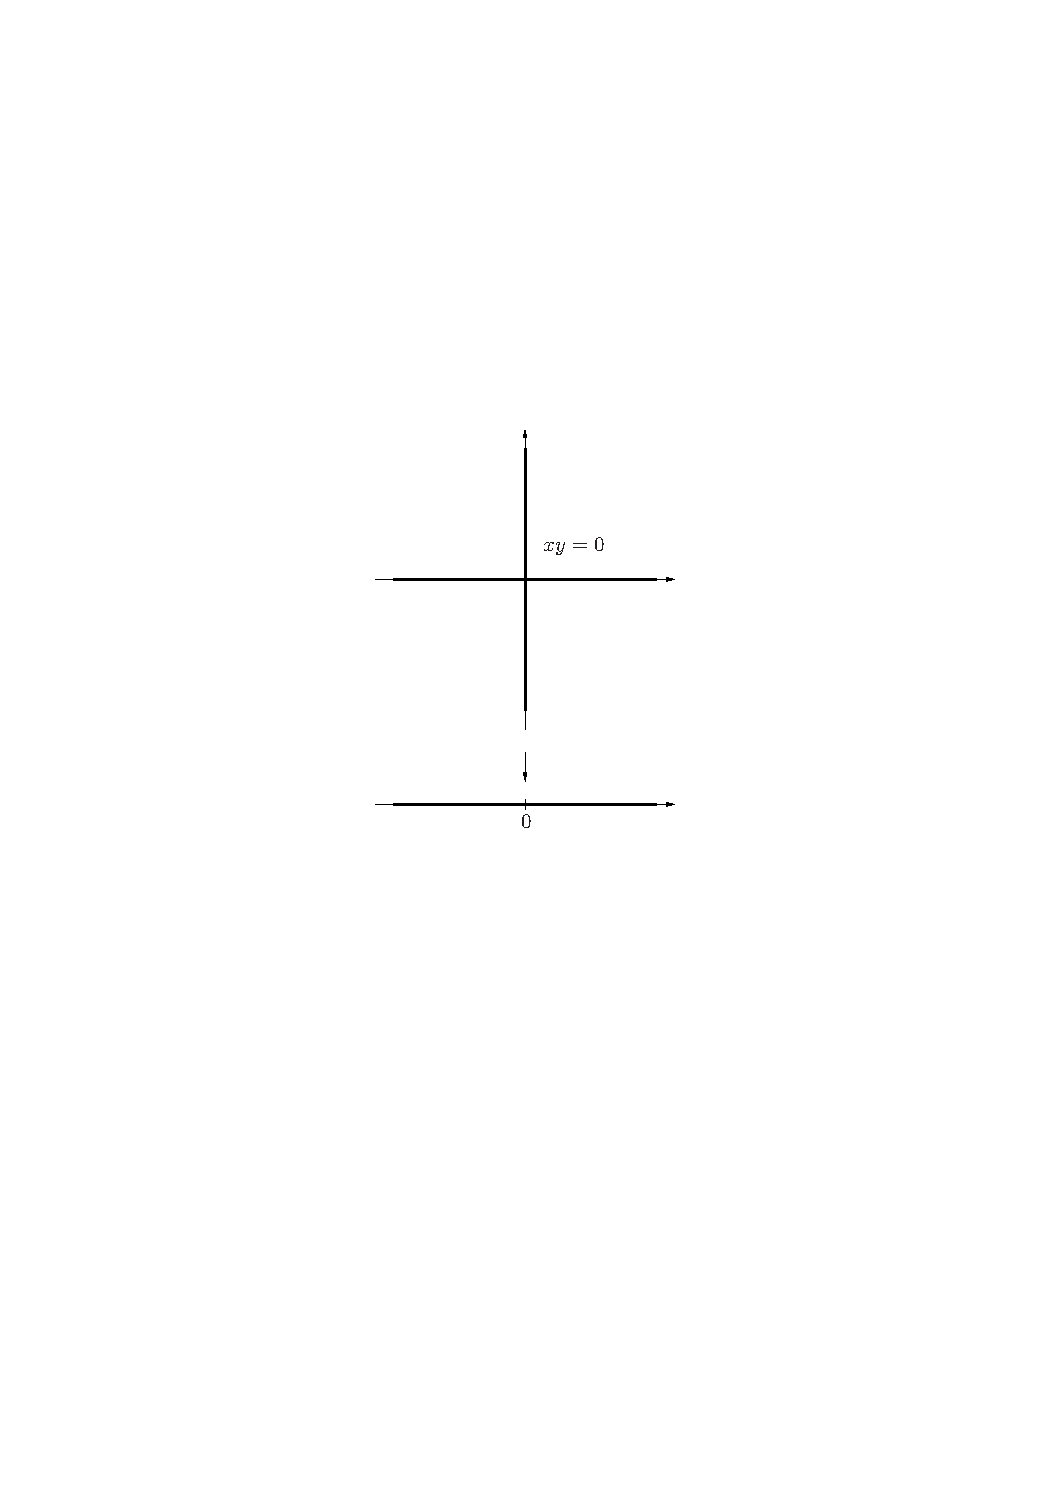
\includegraphics[width=0.3\textwidth]{pictures/flat.pdf}
\end{figure}
In terms of coordinate rings, this map corresponds to the homomorphism of $k$-algebras:
\[k[x]\to\dfrac{k[x,y]}{(xy)}\]
defined by mapping $x$ to the coset $x+(xy)$. This homomorphism defines a $k[x]$-module structure on $k[x, y]/(xy)$, and we can wonder whether the latter is flat. From the geometric point of view, clearly something not flat is going on over the point $x=0$, so we consider the inclusion of the ideal $(x)$ in $k[x]$:
\[\begin{tikzcd}
k[x]\ar[r,hook,"\cdot x"]&k[x]
\end{tikzcd}\]
Tensoring by $k[x,y]/(xy)$, we obtain
\[\begin{tikzcd}
\dfrac{k[x]}{(xy)}\ar[r,"\cdot x"]&\dfrac{k[x]}{(xy)}
\end{tikzcd}\]
which is not injective, because it sends to zero the nonzero coset $y+(xy)$. Therefore $k[x,y]/(xy)$ is not flat as a $k[x]$-module.\par
The term flat was inspired precisely by such geometric examples.
\end{example}
\subsection{The Tor functors}
The \textit{failure of exactness} of the functor $\otimes_{R}N$ is measured by another functor $R$-$\mathsf{Mod}\to R$-$\mathsf{Mod}$, called $\Tor_1^R(-,N)$: if $N$ is flat, then $\Tor^R_1(M,N)=0$ for all modules $M$. In fact if
\[\begin{tikzcd}
0\ar[r]&A\ar[r]&B\ar[r]&C\ar[r]&0
\end{tikzcd}\]
is an exact sequence of $R$-modules, one obtains a new exact sequence after tensoring by any $N$:
\[\begin{tikzcd}
\Tor^R_1(C,N)\ar[r]&A\otimes_{R}N\ar[r]&B\otimes_{R}N\ar[r]&C\otimes_{R}N\ar[r]&0
\end{tikzcd}\]
so if $\Tor^R_1(C,N)=0$, then the module on the left vanishes; thus every short exact sequence ending in $C$ remains exact after tensoring by $N$ in this case. In fact for all $N$ one can continue this sequence with more $\Tor$-modules, obtaining a longer exact complex:
\[\begin{tikzcd}[column sep=small]
\Tor^R_1(A,N)\ar[r]&\Tor^R_1(B,N)\ar[r]&\Tor^R_1(C,N)\ar[r]&A\otimes_{R}N\ar[r]&B\otimes_{R}N\ar[r]&C\otimes_{R}N\ar[r]&0
\end{tikzcd}\]
This is not the end of the story: the complex may be continued even further by invoking new functors $\Tor^R_2(-,N)$, $\Tor^R_3(-,N)$, etc. These are the \textbf{derived functors of tensor}. To \textit{compute} these functors, one may apply the following procedure: given an $R$-module $M$, find a free resolution
\[\begin{tikzcd}
\cdots\ar[r]&R^{\oplus s_2}\ar[r]&R^{\oplus s_1}\ar[r]&R^{\oplus s_0}\ar[r]&M\ar[r]&0
\end{tikzcd}\]
throw $M$ away, and tensor the free part by $N$, obtaining a complex $M_{\bullet}\otimes_{R}N$:
\[\begin{tikzcd}
\cdots\ar[r]&N^{\oplus s_2}\ar[r]&N^{\oplus s_1}\ar[r]&N^{\oplus s_0}\ar[r]&0
\end{tikzcd}\]
(recall again that tensor commutes with colimits, hence with direct sums, therefore $R^{\oplus m}\otimes_{R}N=N^{\oplus m}$); then take the homology of this complex. Astoundingly, this \textit{will not depend $($up to isomorphism$)$ on} the chosen free resolution,
so we can define
\[\Tor_i^{R}(M,N):=H_i(M_{\bullet}\otimes_{R}N)\]
For example, according to this definition $\Tor^R_0(M,N)\cong M\otimes_{R}N$, and $\Tor^R_i(M,N)=0$ for all $i>0$ and all $M$ if $N$ is flat (because then tensoring by $N$ is an exact functor, so tensoring the resolution of $M$ returns an exact sequence, thus with no homology). In fact, this proves a remarkable property of the $\Tor$ functors: if $\Tor^R_1(M,N)=0$ for all $M$, then $\Tor^R_i(M,N)=0$ for all $i>0$ and all modules $M$. Indeed, $N$ is then flat.\par
Since $M\otimes_{R}N$ is canonically isomorphic to $N\otimes_{R}M$ (in the commutative case), we could expect the same to apply to every $\Tor^R_i$: $\Tor^R_i(M,N)$ ought to be canonically isomorphic to $\Tor^R_i(N,M)$ for all $i$. Equivalently, we should be able to compute $\Tor^R_i(M,N)$ as the homology of $M\otimes_{R}N_{\bullet}$, where $N_{\bullet}$ is a free resolution of $N$. This is indeed the case.\par
In fact, we know enough about finitely generated modules over PIDs to get a preliminary sense of what is involved in proving such general facts. Recall that we have been able to establish that every finitely generated module $M$ over a PID $R$ has a free resolution of length $1$:
\[\begin{tikzcd}
0\ar[r]&R^{\oplus m_1}\ar[r]&R^{\oplus m_0}\ar[r]&M\ar[r]&0
\end{tikzcd}\]
This property characterizes PIDs. If
\[\begin{tikzcd}
0\ar[r]&A\ar[r]&B\ar[r]&C\ar[r]&0
\end{tikzcd}\]
is an exact sequence of $R$-modules, it is not hard to see that one can produce compatible resolutions, in the sense that the rows of the following diagram will be exact as well as the columns:
\[
\begin{tikzcd}
&0\ar[d]&0\ar[d]&0\ar[d]&\\
0\ar[r]&R^{\oplus a_1}\ar[d,"\alpha"]\ar[r]&R^{\oplus b_1}\ar[d,"\beta"]\ar[r]&R^{\oplus c_1}\ar[d,"\gamma"]\ar[r]&0\\
0\ar[r]&R^{\oplus a_0}\ar[d]\ar[r]&R^{\oplus b_0}\ar[d]\ar[r]&R^{\oplus c_0}\ar[d]\ar[r]&0\\
0\ar[r]&A\ar[r]\ar[d]&B\ar[r]\ar[d]&C\ar[r]\ar[d]&0\\
&0&0&0&
\end{tikzcd}
\]
Tensor the two free rows by $N$; they remain exact (tensoring commutes with direct sums):
\[
\begin{tikzcd}
0\ar[r]&N^{\oplus a_1}\ar[d,"\alpha\otimes N"]\ar[r]&N^{\oplus b_1}\ar[d,"\beta\otimes N"]\ar[r]&N^{\oplus c_1}\ar[d,"\gamma\otimes N"]\ar[r]&0\\
0\ar[r]&N^{\oplus a_0}\ar[r]&N^{\oplus b_0}\ar[r]&N^{\oplus c_0}\ar[r]&0\\
\end{tikzcd}
\]
Now the columns (preceded and followed by $0$) are precisely the complexes $A_{\bullet}\otimes_{R}N$, $B_{\bullet}\otimes_{R}N$, $C_{\bullet}\otimes_{R}N$ whose homology computes the Tor modules. Applying the snake lemma gives the exact sequence
\[\begin{tikzcd}
0\ar[r]&H_1(A_{\bullet}\otimes_{R}N)\ar[r] &H_1(B_{\bullet}\otimes_{R}N)\rar
\ar[draw=none]{d}[name=X, anchor=center]{}
&H_1(C_{\bullet}\otimes_{R}N)\ar[rounded corners,swap,
to path={ -- ([xshift=2ex]\tikztostart.east)
	|- (X.center) \tikztonodes
	-| ([xshift=-2ex]\tikztotarget.west)
	-- (\tikztotarget)}]{dll}[at end]{\delta}&\\      
&H_0(A_{\bullet}\otimes_{R}N)\rar &H_0(B_{\bullet}\otimes_{R}N)\rar &H_0(C_{\bullet}\otimes_{R}N)\ar[r]&0
\end{tikzcd}\]
which is precisely the sequence of $\Tor$ modules conjured up above.\par
Note that $\Tor^k_i$ vanishes for $i>0$ if $k$ is a field, as vector spaces are flat, and $\Tor^R_i$ vanishes for $i>1$ if $R$ is a PID.
\subsection{Exercise}
$R$ denotes a fixed commutative ring.
\begin{exercise}
Let $M,N$ be $R$-modules, and assume that $N$ is cyclic. Prove that every element of $M\otimes_{R}N$ may be written as a pure tensor.
\end{exercise}
\begin{proof}
Every element in $\otimes_{R}N$ has the form
\[\sum_im_i\otimes n_i=\sum_im_i\otimes(r_in)=\sum_i(r_im_i)\otimes n=(\sum_i r_im_i)\otimes n\]
\end{proof}
\begin{exercise}
Prove by hand $($that is, without appealing to the right-exactness of tensor$)$ that $\Z/n\Z\otimes_{\Z}\Z/m\Z\cong0$ if $m,n$ are relatively prime integers.
\end{exercise}
\begin{proof}
For $\Z/m\Z$, $\Z/n\Z$, We have:
\[m(a\otimes b)=(0\otimes b)=0\cdot(0\otimes b)=0\]
and 
\[n(a\otimes b)=(a\otimes 0)=0\cdot(a\otimes 0)=0\]
since $\gcd(m,n)=1$, there is $u,v\in\Z$ such that 
\[um+vn=1.\]
Then this gives $(a\otimes b)=0$.
\end{proof}
\begin{exercise}
Prove that $R[x_1,\dots,x_n]\otimes_{R}R[y_1,\dots,y_m]\cong R[x_1,\dots,x_n,y_1,\dots,y_m]$.
\end{exercise}
\begin{proof}
For any bilinear function $\theta:R[x_1,\dots,x_n]\times R[y_1,\dots,y_m]\to P$, we have an induced homomorphism:
\[(f,g)\mapsto(fg)\stackrel{\widetilde{\theta}}{\mapsto}\theta(f,g)\for f\in R[x_1,\dots,x_n], g\in R[y_1,\dots,y_m]\]
this is a $R$-linear map. So $R[x_1,\dots,x_n,y_1,\dots,y_m]$ satisfies the universal property of $R[x_1,\dots,x_n]\otimes_{R}R[y_1,\dots,y_m]$.
\end{proof}
\begin{exercise}
Let $S,T$ be commutative $R$-algebras. Verify the following:
\begin{itemize}
\item The tensor product $S\otimes_{R}T$ has an operation of multiplication, defined on pure tensors by $(s_1\otimes t_1)\cdot(s_2\otimes t_2):=s_1s_2\otimes t_1t_2$ and making it into a commutative $R$-algebra.
\item With respect to this structure, there are $R$-algebra homomorphisms $i_S:S\to S\otimes T$, resp., $i_T:T\to S\otimes T$, defined by $i_S(s):=s\otimes1$, $i_T(t):=1\otimes t$.
\item The $R$-algebra $S\otimes_{R}T$, with these two structure homomorphisms, is a coproduct of $S$ and $T$ in the category of commutative $R$-algebras: if $U$ is a commutative $R$-algebra and $f_S:S\to U$, $f_T:T\to U$ are $R$-algebra homomorphisms, then there exists a unique $R$-algebra homomorphism $f_S\otimes f_T$ making the following diagram commute:
\[\begin{tikzcd}
S\ar[rd,swap,"i_S"]\ar[rrrd,bend left=20,"f_S"]&&\\
&S\otimes_{R}T\ar[rr,"f_S\otimes f_T"]&&U\\
T\ar[ru,"i_T"]\ar[rrru,swap,bend right=20,"f_T"]
\end{tikzcd}\]
In particular, if $S$ and $T$ are simply commutative rings, then $S\otimes_{\Z}T$ is a coproduct of $S$ and $T$ in the category of commutative rings.
\end{itemize}
\begin{proof}
Define
\[f_S\otimes f_T(s\otimes t):=f_S(s)f_T(t)\]
this is an $R$-algebra homomorphsim.
\end{proof}
\end{exercise}
\begin{exercise}
Changing the base ring in a tensor may or may not make a difference:
\begin{itemize}
\item Prove that $\Q\otimes_{\Z}\Q\cong\Q\otimes_{\Q}\Q$.
\item Prove that $\C\otimes_{\R}\C\not\cong\C\otimes_{\C}\C$.
\end{itemize}
\end{exercise}
\begin{proof}
$\Q$-$\mathsf{Vect}$ is a full subcategory of $\Z$-$\mathsf{Mod}$, since every $\Z$-linear homomorphism can be extended to be a $\Q$-linear homomorphism.
\end{proof}
\begin{exercise}
Let $R$ be an integral domain, with field of fractions $K$, and let $M$ be a finitely generated R-module. The tensor product $V:= M\otimes_{R}K$ is a $K$-vector space. Prove that $\dim_KV$ equals the rank of $M$ as an $R$-module,
\end{exercise}
\begin{proof}
The scalar product of $V$ is defined to be
\[\dfrac{a}{s}\cdot(m\otimes\dfrac{b}{t}):=m\otimes\dfrac{ab}{st}=(am)\otimes\dfrac{b}{st}\]
it is obvious that basis in $M$ can be transformed into a basis of $V$.
\end{proof}
\begin{exercise}
Let $G$ be a finitely generated abelian group of rank $r$. Prove that $G\otimes_{\Z}\Q\cong\Q^r$.
Prove that for infinitely many primes $p$, $G\otimes_{\Z}(\Z/p\Z)\cong(\Z/p\Z)^r$.
\end{exercise}
\begin{proof}
Since every finite generated abelian group of rank $r$ can be written into $G=\Z^r\oplus T$ where $T$ is a torsion group, we may prove that $T\otimes_{\Z}=0$, then the claim follows from the fact that
\[(\Z^r\oplus T)\otimes_{\Z}\Q\cong (\Z^r\otimes_{\Z}\Q)\oplus(T\otimes_{\Z}\Q)=\Z^r\otimes_{\Z}\Q=\Q^r\]
But this follows from the observation that
\[\dfrac{p}{q}\otimes g=\dfrac{Np}{Nq}\otimes g=\dfrac{p}{q}\otimes Ng=\dfrac{p}{q}\otimes 0=0\]
where $N\in\Ann(T)$.
\end{proof}
\begin{exercise}
Prove that direct sums of flat modules are flat.
\end{exercise}
\begin{proof}
Corollary~\ref{tensor sum}.
\end{proof}
\begin{exercise}
Prove that, according to the definition, $\Tor^R_0(M,N)$ is isomorphic to $M\otimes_RN$.
\end{exercise}
\begin{proof}
$\Tor^R_0(M,N)=H_0(M_{\bullet}\otimes_{R}N)$. For a free resolution of $M$:
\[\begin{tikzcd}
\cdots\ar[r]&R^{\oplus s_2}\ar[r]&R^{\oplus s_1}\ar[r,"\psi"]&R^{\oplus s_0}\ar[r]&M\ar[r]&0
\end{tikzcd}\]
we know that $M=R^{s_0}/\im\psi$. Since $\otimes_{R}N$ is a left-adjoint funtor, it is right exact. So
\[\begin{tikzcd}
R^{\oplus s_1}\otimes_{R}N\ar[r,"\psi\otimes N"]&R^{\oplus s_0}\otimes_{R}N\ar[r]&M\otimes_{R}N\ar[r]&0
\end{tikzcd}\]
is an exact sequence. Since $R^{\oplus s_0}\otimes N/\im(\psi\otimes N)$ is the homology $H_0$, we get the result.
\end{proof}
\begin{exercise}\label{Tor(R/(r),M)}
Prove that for $r\in R$ a non-zero-divisor and $N$ an $R$-module, the module $\Tor^R_1(R/(r),N)$ is isomorphic to the $r$-torsion of $N$, that is, the submodule of elements $n\in N$ such that $rn=0$. $($This is the reason why $\Tor$ is called $\Tor$.$)$
\end{exercise}
\begin{proof}
Consider an exact sequence (the free resolution of $R/(r)$)
\[\begin{tikzcd}
0\ar[r]&(r)\ar[r,"i"]&R\ar[r]&R/(r)\ar[r]&0
\end{tikzcd}\]
Tensoring with $N$ gives an exact sequence
\[\begin{tikzcd}
(r)\otimes_{R}N\ar[r,"i\otimes N"]&N\ar[r]&R/(r)\otimes_{R}N\ar[r]&0
\end{tikzcd}\]
So
\[H_1=\ker(i\otimes N)=\ker(M\stackrel{r}{\to}M)=M_r.\]
\end{proof}
\begin{exercise}
Let $I,J$ be ideals of $R$. Prove that $\Tor^R_1(R/I,R/J)\cong(I\cap J)/IJ$. $($For example, this $\Tor^R_1$ vanishes if $I+J=R$.$)$ Prove that $\Tor^R_i(R/I,R/J)$ is isomorphic to $\Tor^R_{i-1}(I,R/J)$ for $i>1$.
\end{exercise}
\begin{proof}
First, we compute $\Tor^R_1(R,R/J)$. For the free resolution of $R$:
\[\begin{tikzcd}
0\ar[r]&R\ar[r]&R\ar[r]&0
\end{tikzcd}\]
tensoring $R/J$ gives
\[\begin{tikzcd}
0\ar[r]&R\otimes R/J\ar[r]&R\otimes R/J\ar[r]&0
\end{tikzcd}\]
so we find $\Tor_0^R(R,R/J)=R/J$, and $\Tor^R_i(R,R/J)=0$ for $i>0$.\par
Now for the exat sequence
\[\begin{tikzcd}
0\ar[r]&I\ar[r]&R\ar[r]&R/I\ar[r]&0
\end{tikzcd}\]
tensoring with $R/J$ gives a new exact sequence:
\[\begin{tikzcd}[column sep=small]
\Tor_1^R(R,R/J)\ar[r]&\Tor_1^R(R/I,R/J)\ar[r]&I\otimes R/J\ar[r]&R\otimes R/J\ar[r]&R/I\otimes R/J\ar[r]&0
\end{tikzcd}\]
With $\Tor_1^R(R,R/J)=0$, $I\otimes R/J=I/IJ$, $R\otimes R/J=R/J$, $R/I\otimes R/J=R/(I+J)$, this becomes
\[\begin{tikzcd}
0\ar[r]&\Tor_1^R(R/I,R/J)\ar[r]&\dfrac{I}{IJ}\ar[r,"\psi"]&R/J\ar[r]&\dfrac{R}{I+J}\ar[r]&0
\end{tikzcd}\]
so we have $\Tor_1^R(R/I,R/J)\cong\ker\psi$. Since $\psi$ maps $I$ to $R$, its kernel should be
\[\ker\psi=\{i+IJ\mid i\in J\}=\dfrac{I\cap J}{IJ}\]
so the first claim follows.\par
\end{proof}
\begin{exercise}
Let $M,N$ be modules over a PID $R$. Prove that $\Tor^R_i(M,N)=0$ for $i\geqslant2$. $($Assume $M,N$ are finitely generated, for simplicity.$)$
\end{exercise}
\begin{proof}
The resolution of finitely generated over a module has length $\leqslant 1$.
\end{proof}
\begin{exercise}\label{flat iff free}
Let $R$ be an integral domain. Prove that a cyclic $R$-module is flat if and only if it is free.
\end{exercise}
\begin{proof}
Let $M=\langle m\rangle$ be a cyclic module. If $M$ is free, then it has a free resolution
\[\begin{tikzcd}
0\ar[r]&R\ar[r]&\langle m\rangle\ar[r]&0
\end{tikzcd}\]
tensoring with any module $M$, it is clear that $\Tor^R_i(M,N)=0$ fro $i>0$, so $M$ is flat.\par
Conversely, if $M$ is flat, since $M\cong R/I$ for some ideal $I$, $R$ is free if and only if it is torsion free. For any fixed $r\in R$, consider the map $\psi:R\to R,\quad x\mapsto rx$. If $r\neq0$, since $R$ is an integral domain, $\psi$ is injective. Now $M$ is flat, so $\psi\otimes M$ is also injective. But $\psi\otimes M$ has the expression:
\[\psi\otimes M:R\otimes M\to R\otimes M,\quad x\otimes m\mapsto rx\otimes m\]
so it can be viewed as a map $\psi\otimes M:M\to M$ sending $m$ to $rm$. Since this is injective for any nonzero $r\in R$, we concluede $M$ is torsion free, hence free.
\end{proof}
\begin{exercise}\label{flat crit}
The following criterion is quite useful.
\begin{itemize}
\item Prove that an $R$-module $M$ is flat if and only if every monomorphism of $R$ modules $A\to B$ induces a monomorphism of $R$-modules $A\otimes M\to B\otimes M$.
\item Prove that it suffices to verify this condition for all finitely generated modules $A$, $B$.
\item Prove that it suffices to verify this condition when $B=R$ and $A=I$ is an ideal of $R$.
\item Deduce that an $R$-module $M$ is flat if and only if the natural homomorphism $I\otimes_{R}M\to IM$ is an isomorphism for every ideal $I$ of $R$.
\end{itemize}
If you believe in $\Tor$'s, now you can also show that an $R$-module $M$ is flat if and only if $\Tor^R_1(R/I,M)=0$ for all ideals $I$ of $R$.
\end{exercise}
\begin{proof}
\mbox{}
\begin{itemize}
\item This is obvious.
\item An element $\sum_ia_i\otimes m_i\in A\otimes_{R}M$ goes to zero in $B\otimes_{R}M$ if the
corresponding element $\sum_i(f(a_i),m_i)$ equals a combination of the relations defining $B\otimes_{R}M$ in the free $R$-module $F^R(B\times M)$. This will be an identity involving only finitely many elements of $A$ and $B$; hence we should only consider the submodule $N$ of $A$ and $S$ of $B$ generated by these elements and the restricted morphism from $N\otimes M\to S\otimes M$. If the condition is satisfied by finite generated modules, then this will be a monomorphism, so we get $\sum_ia_i\otimes m_i=0$ as needed.
\item We may now assume that $B$ is finitely generated. Find submodules $B_j$ such that $A=B_0\sub B_1\sub\cdots\sub B_r=B$, with each $B_j/B_{j-1}$ cyclic. Reduce to verifying that $A\otimes M$ injects in $B\otimes_{R} M$ when $B/A$ is cyclic, hence $\cong R/I$ for some ideal $I$. Now consider the exact sequence
\[\begin{tikzcd}
\Tor^R_1(B/A,M)\ar[r]&A\otimes M\ar[r]&B\otimes M\ar[r]&B/A\otimes M\ar[r]&0
\end{tikzcd}\]
the claim follows if and only if $\Tor^R_1(B/A,M)=\Tor^R_1(R/I,M)=0$.
\item $I\otimes M\to IM$ is clearly surjective. $M$ is flat iff $\Tor^R_1(R/I,M)=0$, if and only if $I\otimes M\to IM$ is injective.
\end{itemize}
\end{proof}
\begin{exercise}\label{PID flat iff torsion}
Let $R$ be a PID. Prove that an $R$-module $M$ is flat if and only if it is torsion free.\par
Geometrically, this says roughly that an algebraic set fails to be flat over a nonsingular curve if and only if some component of the set is contracted to a point.
\end{exercise}
\begin{proof}
Let $T$ be the torsion part of $M$, and let $r\in\Ann(x)$ for some $x\in M$. Then by Exercise~\ref{Tor(R/(r),M)}, $\Tor(R/(r),M)=M_r$ the $r$-torsion submodule of $M$. Since by Exercise~\ref{flat crit}, $M$ is flat iff this Tor is zero, we conclude that $M$ is flat iff $M$ is torsion-free.
\end{proof}
\begin{exercise}\label{local Tor}
Let $M,N$ be $R$-modules, and let $S$ be a multiplicative subset of $R$. Use the definition of $\Tor$ to show $S^{-1}\Tor^R_i(M,N)\cong\Tor^{S^{-1}R}_i(S^{-1}M,S^{-1}N)$.\par
Use this fact to give a leaner proof that flatness is a local property.
\end{exercise}
\begin{proof}
For a resolution of $M$:
\[\begin{tikzcd}
\cdots\ar[r]&R^{\oplus s_2}\ar[r]&R^{\oplus s_1}\ar[r]&R^{\oplus s_0}\ar[r]&M\ar[r]&0
\end{tikzcd}\]
tensoring with $N$ gives the computation of $\Tor^R_i(M,N)$:
\[\begin{tikzcd}
\cdots\ar[r]&N^{\oplus s_2}\ar[r]&N^{\oplus s_1}\ar[r]&N^{\oplus s_0}\ar[r]&0
\end{tikzcd}\]
By Exercise~\ref{locali exact}, $S^{-1}H_i(M_{\bullet}\otimes_{R}N)\cong H_i(S^{-1}(M_{\bullet}\otimes_{R}N))$.\par
First we check that localization commutes with direct sum. That is, $S^{-1}(R^{\oplus r})=(S^{-1}R)^{\oplus r}$. In fact, we have a natural isomorphism:
\[\theta:\dfrac{(a_1,\dots,a_r)}{s}\mapsto\Big(\dfrac{a_1}{s},\dots,\dfrac{a_r}{s}\Big)\]
This is surjective since for any element in $(S^{-1}R)^{\oplus r}$:
\[\Big(\dfrac{a_1}{s_1},\dots,\dfrac{a_r}{s_r}\Big)=\Big(\dfrac{a_1\prod_{i\neq 1}s_i}{s_1\cdots s_r},\dots,\dfrac{a_r\prod_{i\neq r}s_i}{s_1\cdots s_r}\Big)=\theta\Big(\dfrac{a_1\prod_{i\neq 1}s_i,\dots,a_r\prod_{i\neq r}s_i}{s_1\cdots s_r}\Big)\]
The injectivity follows from
\[\Big(\dfrac{a_1}{s},\dots,\dfrac{a_r}{s}\Big)=0\iff (\exists t_i\in S)\ t_ia_i=0\Rightarrow \dfrac{(a_1,\dots,a_r)}{s}=\dfrac{(a_1t_1\prod_{i\neq 1}t_i,\dots,a_rt_r\prod_{i\neq r}t_i)}{s\prod_it_i}=0\]
With this, apply localization gives
\[S^{-1}(N^{\oplus s})=S^{-1}(R^{\oplus s}\otimes_{R}N)=(S^{-1}R^{\oplus s})\otimes_{S^{-1}R}N\cong (S^{-1}R)^{\oplus s}\otimes_{R}N\cong(S^{-1}R)^{\oplus s}\otimes_{S^{-1}R}(S^{-1}N)\]
where we use Exercise~\ref{local tensor}. Now the claim follows from that localizing the sequence
\[\begin{tikzcd}
\cdots\ar[r]&R^{\oplus s_2}\ar[r]&R^{\oplus s_1}\ar[r]&R^{\oplus s_0}\ar[r]&M\ar[r]&0
\end{tikzcd}\]
gives a resolution of $S^{-1}M$.
\end{proof}
\begin{exercise}\label{flat exact sequence}
Let
\[\begin{tikzcd}
0\ar[r]&M\ar[r]&N\ar[r]&P\ar[r]&0
\end{tikzcd}\]
be an exact sequence of $R$-modules, and assume that $P$ is flat.
\begin{itemize}
\item Prove that $M$ is flat if and only if $N$ is flat.
\item Prove that for all R-modules Q, the induced sequence
\[\begin{tikzcd}
0\ar[r]&M\otimes_{R}Q\ar[r]&N\otimes_{R}Q\ar[r]&P\otimes_{R}Q\ar[r]&0
\end{tikzcd}\]
is exact.
\end{itemize}
\end{exercise}
\begin{proof}
\mbox{}
\begin{itemize}
\item For any $R$-module $Q$, the sequence
\[\begin{tikzcd}
0\ar[r]&\Tor^R_1(M,Q)\ar[r]&\Tor^R_1(N,Q)\ar[r]&\Tor^R_1(P,Q)\ar[r]&0
\end{tikzcd}\]
is also exact. Since $\Tor^R_1(P,Q)=0$, we get the claim.
\item Tensoring $Q$ gives an exact sequence:
\[\begin{tikzcd}
\Tor^R_1(P,Q)\ar[r]&M\otimes_{R}Q\ar[r]&N\otimes_{R}Q\ar[r]&P\otimes_{R}Q\ar[r]&0
\end{tikzcd}\]
since $P$ is flat, $\Tor^R_1(P,Q)=0$, we get the claim.
\end{itemize}
\end{proof}
\begin{exercise}\label{local flat iff free}
Let $R$ be a commutative Noetherian local ring with $(single)$ maximal ideal $\mathfrak{m}$, and let $M$ be a finitely generated flat $R$-module.
\begin{itemize}
\item Choose elements $m_1,\dots,m_r\in M$ whose cosets mod $\mathfrak{m}M$ are a basis of $M/\mathfrak{m}M$ as a vector space over the field $R/\mathfrak{m}$. By Nakayama's lemma, $M=\langle m_1,\dots,m_r\rangle$.
\item Obtain an exact sequence
\[\begin{tikzcd}
0\ar[r]&N\ar[r]&R^{\oplus r}\ar[r]&M\ar[r]&0
\end{tikzcd}\]
where $N$ is finitely generated.
\item Prove that this sequence induces an exact sequence
\[\begin{tikzcd}
0\ar[r]&N/\mathfrak{m}N\ar[r]&(R/\mathfrak{m})^{\oplus r}\ar[r]&M/\mathfrak{m}M\ar[r]&0
\end{tikzcd}\]
\item Deduce that $N=0$.
\item Conclude that $M$ is free.
\end{itemize}
Thus, a finitely generated module over a (Noetherian) local ring is flat if and only if it is free.
\end{exercise}
\begin{proof}
\mbox{}
\begin{itemize}
\item Since $M$ is generated by $m_1,\dots,m_r$, there is a epimorphism from $R^{\oplus r}$ to $M$.
\item By Exercise~\ref{flat exact sequence}, tensoring with $R/\mathfrak{m}$ gives the exact sequence. Since we have $(R/I)\otimes N\cong N/IN$.
\item Since $M/\mathfrak{m}M$ is a vector space over $R/\mathfrak{m}$ with basis $m_1+\mathfrak{m}M,\dots,m_r+\mathfrak{m}M$, we must have $N/\mathfrak{m}N=0$. Then $N=\mathfrak{m}M$, by Nakayama's Lemma, $N=0$.
\item Since $N=0$, we get $M\cong R^{\oplus r}$.
\end{itemize}
\end{proof}
\begin{exercise}
Let $R$ be a commutative Noetherian ring, and let $M$ be a finitely generated $R$-module. Prove that
\[M\text{ is flat}\iff \Tor^R_1(M,R/\mathfrak{m})=0\text{ for every maximal ideal $\mathfrak{m}$ of $R$}\]
\end{exercise}
\begin{proof}
On direction is trivial. So we assume that $\Tor^R_1(M,R/\mathfrak{m})=0$ for every maximal ideal $\mathfrak{m}$. Since we only need to show $M_{\mathfrak{m}}$ is flat for every maximal ideal $\mathfrak{m}$, we localize $\Tor$ to get
\[\Tor^{R_\m}_1(M_\m,R_\m/\m R_\m)=0\]
Hence we may assume $A$ is local. Then as in the proof of Proposition~\ref{local flat iff free}, we can show $M_\m$ is free, hence is flat.
\end{proof}
\section{Base change}
In this section, we connect the modules on two different rings, i.e., we consider the functors between two categories $R$-$\mathsf{Mod}$ and $S$-$\mathsf{Mod}$. To fit further applications of this topic, we are \textit{not} assuming that $R$ and $S$ are commutative. Thus we have to deal with left and right modules.
\subsection{Tensor products over noncommutative ring}
Let $R$ be a ring (not necessarily commutative), and $M$ be a right $R$-module, $N$ a left $R$-module. We indicate this situation by writing $M_R$ and $_{R}N$ in the respective cases. Let $P$ be an abelian group. A $\Z$-bilinear map $f:M\times N\to P$ is \textbf{$\bm{R}$-balanced} or an \textbf{$\bm{R}$-balanced product} if for any $r\in R$, $m\in M$, $n\in N$ we have
\[f(mr,n)=f(m,rn).\]
In this situation, we denote the $R$-balanced map by $(P,f)$. If $(L,g)$ is a second one, then we define a morphism from $(P,f)$ to $(L,g)$ to be a homomorphism $\varphi$ of the additive group $P$ into the additive group $L$ such that for any $m\in M$, $n\in N$ we have
\[g(m,n)=\varphi(f(m,n)).\]
That is, we require the following diagram to commute:
\[\begin{tikzcd}[column sep=small, row sep=small]
&P\ar[dd,"\varphi"]\\
M\times N\ar[rd,swap,"g"]\ar[ru,"f"]&\\
&L
\end{tikzcd}\]
Therefore the balanced maps from $M\times N$ form a category, which we may denote by $\mathcal{B}(M,N)$. We can now introduce the following definition.
\begin{definition}
Then \textbf{tensor product} of $M_{R}$ and $_{R}N$ is a balanced product $(M\otimes_RN,\otimes)$ such that if $(P,f)$ is any balanced product of $M_{R}$ and $_{R}N$, then there exists a unique morphism of $(M\otimes_{R}N,\otimes)$ to $(P,f)$:
\[\begin{tikzcd}[column sep=small, row sep=small]
&M\otimes_{R}N\ar[dd,"\exists!"]\\
M\times N\ar[rd,swap,"f"]\ar[ru,"\otimes"]&\\
&P
\end{tikzcd}\]
In other words, $(M,\otimes_{R}N,\otimes)$ is the initial object in the category $\mathcal{B}(M,N)$.
\end{definition}
The tensor product defined above can be constructed similarly to the commutative case. We now establish them in detail.
\begin{proposition}
The tensor product $M\otimes_RN$ exists for any modules $M_{R}$ and $_{R}N$.
\end{proposition}
\begin{proof}
Consider the free abelian group $\Z^{\oplus(M\times N)}$. Let $K$ be the subgroup that is generated by elements of the form
\[\begin{array}{c}
(m,n_1+n_2)-(m,n_1)-(m,n_2)\\
(m_1+m_2,n)-(m_1,n)-(m_2,n)\\
(rm,n)-(m,rn)
\end{array}\]
with $m,m_1,m_2\in M$, $n,n_1,n_2\in N$, $r\in R$. It is now easy to check that the quotient $\Z^{\oplus(M\times N)}/K$, together with the map
\[\otimes:M\times N\to \Z^{\oplus(M\times N)}/K,\quad(m,n)\mapsto(m,n)+K\]
satisfies the condition required.
\end{proof}
We simplify the notation to $M\otimes N$ or $M\otimes_RN$ if we need to specify the ring $R$, and we speak of the tensor product of $M$ and $N$. Now suppose we have module homomorphisms $f:M\to M'$ and $g:N\to N'$. Then we have the map
\[M\times N\to M'\otimes N',\quad (m,n)\mapsto f(m)\otimes g(n)\]
which satisfies the conditions for a balanced product of $M$ and $N$ by the definition of tensor product. Hence we have a unique homomorphism of $f\otimes g:M\otimes N\to M'\otimes N'$ such that
\[(f\otimes g)(m,n)=f(m)\otimes g(n).\]
Suppose next that we have homomorphisms $f':M'\to M''$ and $g':N'\to N''$, then it is clear that
\[(f'\circ f)\otimes(g'\circ g)(m\otimes n)=(f'(f(m)))\otimes(g(g'(n))),\]
and therefore
\[(f'\circ f)\otimes(g'\circ g)=(f'\otimes f)\otimes(g'\circ g).\]
Since $(\id_M\otimes\id_N)(m\otimes n)=m\otimes n$, we have $\id_M\otimes\id_N=\id_{M\otimes N}$. These results amount to saying we have defined a functor $\mathsf{Mod}\text{-$R$}\times\text{$R$-}\mathsf{Mod}\to\mathsf{Ab}$. We shall denote this functor as $\otimes_R$.\par
We shall now fix one of the arguments in the functor $\otimes_R$ and study the resulting functors of one variable. Let $M$ be a fixed right $R$-module. Then we define the functor $M\otimes_R$ (or $M\otimes$) from $R$-$\mathsf{Mod}$ to $\Z$-$\mathsf{Mod}$ by specifying that for any left $R$-module $N$ and any homomorphism $g:N\to N'$ of left $R$-modules, we have
\[(M\otimes_R)(N)=M\otimes_RN,\quad (M\otimes_R)(g)=\id_M\otimes g.\]
From this definition, the functorial properties are easy to verify. In a similar manner, any left module defines a functor $\otimes_RN$ (or $\otimes N$) from $\mathsf{Mod}$-$R$ to $\mathsf{Mod}$-$\Z$ by
\[(\otimes_RN)(M)=M\otimes_RN,\quad (N\otimes_R)(f)=f\otimes\id_N.\]
for $f:M\to M'$ in $\mathsf{Mod}$-$R$. The properties of $M\otimes_R$ and $\otimes_RN$ are similar to the commutative case. To simplify the discussion, we will establish them for tensor product of bimodules.
\begin{example}
Let $R^{op}$ be the opposite ring of $R$ and regard a right (left) $R$-module as a left (right) $R^{op}$-module in the usual way. Consider the map
\[s:M\times N\to N\times M,\quad (m,n)\mapsto(n,m).\]
If $f:N\times M\to P$ is a $R^{op}$-balanced product, then
\[(f\circ s)(m\cdot r,n)=f(n,m\cdot r)=f(n,rm=f(nr,m)=f(r\cdot n,m)=(f\circ s)(m,r\cdot n).\]
Therefore $f\circ s$ is a $R$-balanced map, and we get a map $f^s:M\otimes N\to P$. Take $P=N\otimes_{R^{op}}M$, we get a map
\[\otimes^s:M\otimes_{R}N\to N\otimes_{R^{op}}M,\quad m\otimes n\mapsto n\otimes m.\]
This is clearly an isomorphism, therefore we get $M\otimes_{R}N\cong N\otimes_{R^{op}}M$ as groups.
\end{example}
\subsection{Bimodules}
Let $M$ be a right $R$-module and let $S=\End_R(M)$. Then $M$ can be regarded as a left $S$-module if we define $fx$ for $f\in S$, $x\in M$, to be the image of $m$ under the map $f$. Since $f$ is a homomorphism of the additive group of $M$, we have $f(x+y)=f(x)+f(y)$, and by definition of the sum and product of homomorphisms, we have $(f+g)x=f(x)+g(x)$ and $(fg)x=f(gx)$ if $f,g\in S$. Clearly also $\id x=x$ so $M$ is a left $S$-module. Also the definition of module homomorphism gives the relation
\[(fx)r=f(x)r=f(xr).\]
for $x\in M$, $r\in R$, $f\in S$. This associativity connects the given right $R$-module structure with the left $S$-module structure of $M$. Similarly, if $M$ is a left $R$-module, then by acting homomorphisms on the right:
\[xf:=f(x)\]
we see that $M$ can be made into a right $S$-module. More generally, we now introduce the following definition.
\begin{definition}
Let $R$ and $S$ be rings. An $(R,S)$-\textbf{bimodule} is an abelian group $M$ endowed with compatible $R$-module and $S$-module structures, in the sense that
\[r(xs)=(rx)s\]
for any $r\in R$, $s\in S$, $x\in M$.
\end{definition}
The foregoing considerations show that if $M$ is a right $R$-module, then $M$ can be regarded in a natural way as an $(S,R)$-bimodule for $S=\End_R(M)$.
\begin{example}[\textbf{Examples of bimodules}]
\mbox{}
\begin{itemize}
\item[(a)] Let $R$ be commutative. Then any right $R$-module $M$ can be regarded also as a left $R$-module by putting $rx=xr$, $r\in R$, $x\in M$. It is often advantageous to regard $M$ as an $(R,R)$-bimodule. The associativity condition $r(xr')=(rx)r'$ is an immediate consequence of the commutativity of $R$.
\item[(b)] Again let $R$ be commutative and let $\varphi$ be an automorphism of $R$. If $M$ is a right $R$-module, $M$ becomes a left $R$-module by defining $rx=\varphi(r)(x)$. This action together with the given right action makes $M$ an $(R,R)$-bimodule.
\item[(c)] Any right $R$-module can be regarded as a $(\Z,R)$-bimodule by defining $nx$ for $n\in\Z$ in the usual way. Similarly, any left $R$-module becomes an $(R,\Z)$-bimodule. In this way the theory of one-sided modules can be subsumed in that of bimodules.
\item[(d)] If $R$ is a ring, we have the left module $_{R}R$ and the right module $R_{R}$. Since we have the associative law $(rx)s=r(xs)$, we can put the two module structures together to obtain a bimodule.
\end{itemize}
\end{example}
If $M$ is a right $R$-module and $N$ is a left $R$-module, then the tensor product $M\otimes_{R}N$ acquires an $\Z$-module structure: define the action of $s,t\in\Z$ on pure tensors $m\otimes n$ by
\[s(m\otimes n)t:=(sm)\otimes(tn)\]
and extend to all tensors by linearity. More generally, if $_{Q}M_{R}$ and $_{R}N_{S}$ are bimodules, then the tensor product $M\otimes_RN$ has a $(Q,S)$-bimodule structure which is defined by
\[q(m\otimes n)s=(qm)\otimes(ns)\]
for $q\in Q$, $s\in S$.\par
With this observation, we now consider the balanced products of bimodules. Let $_{Q}M_{R}$, $_{R}N_{S}$ and $_{Q}P_{S}$ be bimodules. A $R$-balanced map $f:M\times N\to P$ is called \textbf{$\bm{(Q,R,S)}$-balanced} or a \textbf{$\bm{(Q,R,S)}$-balanced product} if for $q\in Q$ and $s\in S$ we have
\[f(qx,ys)=qf(x,y)s.\]
If $(L,g)$ is another such map, then a morphism from $(P,f)$ to $(L,g)$ is a $(Q,S)$-homomorphism from $P$ to $L$ such that $\varphi\circ f=g$. In this way we get a category $\mathbf{Bil}(M,N)$.\par
From the argument above, we see $M\times N\to M\otimes_RN$ is $(Q,R,S)$-balanced. We may also define the tensor product of $_{Q}M_{R}$ and $_{R}N_{S}$ to be the initial object in the category $\mathbf{Bil}(M,N)$, but it is clear that it is isomorphic to $M\otimes_RN$.\par
Similarly, be defining tensor product of morphisms, we get a functor
\[\otimes:(Q,R)\text{-}\mathsf{Mod}\times(R,S)\text{-}\mathsf{Mod}\to(Q,S)\text{-}\mathsf{Mod}.\]
Now we give some properties of the tensor product.
\begin{proposition}
Let $(M_i)_{i\in I}$ be $(Q,R)$-bimodules and $(N_j){j\in J}$ be $(R,S)$-bimodules. Then there are canonical $(Q,S)$-homomorphisms
\[\begin{tikzcd}
(\prod_{i\in I}N_i)\otimes_R(\prod_{j\in J}N_j)\ar[r]&\prod_{(i,j)\in I\times J}M_i\otimes_RN_j\\
(\bigoplus_{i\in I}N_i)\otimes_R(\bigoplus_{j\in J}N_j)\ar[u,hook]\ar[r,"\cong"]&\bigoplus_{(i,j)\in I\times J}M_i\otimes_RN_j\ar[u,hook]
\end{tikzcd}\]
\end{proposition}
\begin{proof}
Note there is a $(Q,S)$-balanced map
\[\prod_{i\in I}M_i\times\prod_{j\in J}N_j\to\prod_{(i,j)\in I\times J}M_i\otimes N_j,\quad((x_i)_{i},(y_j)_{j})\mapsto(x_i\otimes y_j)_{i,j}\]
Since the restriction of this map on $\bigoplus_{i\in I}M_i\times\bigoplus_{j\in J}N_j$ has image in $\bigoplus_{(i,j)}M_i\otimes_RN_j$, we get the claimed maps. Let $\Phi$ be the homomorphism on the direct sum.\par
Let $P$ be a $(Q,S)$-bimodule, then the following diagram is easy to verify:
\[\begin{tikzcd}
\Hom((\bigoplus_{i\in I}N_i)\otimes_R(\bigoplus_{j\in J}N_j),P)\ar[r,"\cong"]&\mathcal{B}(\bigoplus_{i}M_i,\bigoplus_jN_j;P)\ar[d,"\cong"]\\
&\prod_{i,j}\mathcal{B}(M_i,N_j;P)\\
\Hom(\bigoplus_{(i,j)\in I\times J}M_i\otimes_RN_j,P)\ar[uu,"\Phi^*"]\ar[r,"\cong"]&\prod_{i,j}\Hom(M_i\otimes_RN_j,P)\ar[u,swap,"\cong"]
\end{tikzcd}\]
This proves that $\Phi$ is an isomorphism.
\end{proof}
\begin{proposition}
Let $_{Q}M_{R}$, $_{R}N_{S}$, $_{S}L_{T}$ be bimodules, then there is a canonical isomorphism
\[M\otimes_R(N\otimes_SL)\to (M\otimes_RN)\otimes_SL,\quad x\otimes(y\otimes z)\to(x\otimes y)\otimes z.\]
\end{proposition}
\begin{proof}
To simplify the notation, we let $Q=T=\Z$. Let $P$ be a $(Q,T)$-bimodule then we have
\[\Hom((M\otimes_RN)\otimes_SL,P)=\mathcal{B}((M\otimes_RN)\times_SL;P)\]
\[\Hom(M\otimes_R(N\otimes_SL),P)=\mathcal{B}(M\times_R(N\otimes_SL);P)\]
We will show that both sets on the right are isomorphic to the group of  balanced maps from $M\times N\times N$ to $P$: that is, a $\Z$-multilinear map $f:M\times N\times N\to P$ such that for any $x\in M,y\in N,z\in L$ we have 
\begin{itemize}
\item[(a)] $f(xr,y,sz)=f(x,rys,z)$ with $r\in R,s\in S$.
\item[(b)] $f(qx,y,zt)=qf(x,y,z)t$ with $q\in Q,t\in T$.
\end{itemize}
In fact, given such a map $f$, for any fixed $z\in Z$ the map $f(\cdot,\cdot,z)$ is in $\mathcal{B}(M,N;P)$, and so there is a homomorphism $F(\cdot,z):M\otimes N\to P$ such that $f(x,y,z)=F(x\otimes y,z)$. Now by varying $z$, we have
\begin{align*}
F(x\otimes y,z+z')&=F(x\otimes y,z)+F(x\otimes y,z'),\\
F(x\otimes y,sz)&=f(x,y,sz)=f(x,ys,z)=F(x\otimes ys,z)=F((x\otimes y)s,z),\\
F(q(x\otimes y),zt)&=F(qx\otimes y,zt)=f(qx,y,zt)=qf(x,y,z)t=qF(x\otimes y,z)t.
\end{align*}
Therefore $F\in\mathcal{B}(M\otimes_RN,L;P)$. This then gives a morphism $\varphi:(M\otimes_RN)\otimes_SL\to P$ such that
\[\varphi((x\otimes y)\otimes z)=f(x,y,z).\]
The construction given above can be reversed, so that we see the correspondence
\[\mathcal{B}((M\times_RN)\otimes_SL;P)\Leftrightarrow\{\text{balanced maps $f:M\times N\times L\to P$}\},\]
and similarly
\[\mathcal{B}(M\times_R(N\otimes_SL);P)\Leftrightarrow\{\text{balanced maps $f:M\times N\times L\to P$}\}.\]
Moreover, if $f:M\times N\times L\to P$ is balanced, then the corresponding morphisms are given by
\[\varphi((x\otimes y)\otimes z)=f(x,y,z)=\psi(x\otimes(y\otimes z)).\]
Therefore the claimed isomorphism is established.
\end{proof}
\begin{proposition}\label{tensor product unit}
Let $_{Q}M_{R}$ and $_{R}N_{S}$ be bimodules.
\begin{itemize}
\item[(a)] The map $\eta_M:m\mapsto m\otimes 1$ is an isomorphism of $M$ regarded as a $(Q,R)$-bimodule with $M\otimes_RR$. Moreover, $M\to\eta_M$ is a natural isomorphism of the forgetful functor from $(Q,R)$-$\mathsf{Mod}$ to $Q$-$\mathsf{Mod}$ with the functor $\otimes_RR$.
\item[(b)] The map $\epsilon_N:n\mapsto 1\otimes n$ is an isomorphism of $N$ regarded as a $(R,S)$-module with $R\otimes_RN$. Moreover, $N\to\epsilon_N$ is a natural isomorphism of the forgetful functor from $(R,S)$-$\mathsf{Mod}$ to $\mathsf{Mod}$-$S$ with the functor $R\otimes_R$.
\end{itemize}
\end{proposition}
\begin{proof}
We only do $(a)$, and $(b)$ is done similarly. Clearly $\eta_M$ is a $\Z$-homomorphism. To show that it is a $(Q,R)$-homomorphism, we note that
\[\eta_M(qmr)=qmr\otimes 1=qm\otimes r=q(m\otimes 1)r=q\eta_M(m)r.\]
On the other hand, for $r\in R$ and $m\in M$, the map
\[M\times R\to M,\quad (m,r)\mapsto mr\]
is a $(Q,R,S)$-balanced product of $M$ and $R$. Hence we have a $(Q,S)$-homomorphism $\varphi_M$ of $M\otimes_RR$ into $M$ such that $\varphi_M(m\otimes r)=mr$.
\[\begin{tikzcd}[column sep=small, row sep=small]
&M\otimes_{R}R\ar[dd,"\varphi_M"]\\
M\times R\ar[rd,swap]\ar[ru]&\\
&M
\end{tikzcd}\]
It is clear that $\varphi_M\circ\eta_M=\id_M$ and $\eta_M\circ\varphi_M=\id_{M\otimes_RR}$. Hence the first assertion is valid. The second assertion is an immediate consequence of the definitions.\end{proof}
Now we consider the adjoint condition for tensor and hom. For this, we first need some conventions. Let $R$ be a ring. For left $R$-modules $_{R}M$ and $_{R}N$, we let $\Hom_R({_{R}M},{_{R}N})$ act on $M$ by
\[\Hom_R({_{R}M},{_{R}N})\ni f:m\mapsto mf\in N\]
for $f\in\Hom_R(_{R}M,_{R}N)$. Similarly, for right $R$-modules $M_{R}$ and $N_{R}$, we act $\Hom_R(M_{R},N_{R})$ on the right:
\[\Hom_R(M_{R},N_{R})\ni f:m\mapsto fm\in N.\]
Similarly to the tensor product, we can make $\Hom_R({_{R}M},_{R}N)$ and $\Hom_R(M_{R},N_{R})$ into bimodules.
\begin{proposition}\label{bimodule Hom set is bimodule}
Let $Q,R,S$ be rings.
\begin{itemize}
\item Let $_{R}M_{Q}$ and $_{R}N_{S}$ be bimodules, then the additive group $\Hom_{R}({_{R}M},{_{R}N})$ has a natural $(Q,S)$-bimodule structure which is defined by
\[qfs:m\mapsto((mq)f)s\]
where $q\in Q,s\in S$ and $f\in\Hom_{R}({_{R}M},{_{R}N})$.
\item Let $_{Q}M_{R}$ and $_{S}N_{R}$ be bimodules, then the additive group $\Hom_{R}({M_{R}},{N_{R}})$ has a natural $(S,Q)$-bimodule structure which is defined by
\[sfq:m\mapsto s(f(qm))\]
where $s\in S,q\in Q$ and $f\in\Hom_{R}({M_{R}},{N_{R}})$.
\end{itemize}
\end{proposition}
\begin{proof}
These definitions are natural in view of associativity. For example, under the first definition,
\[(rm)(qfs)=(rmq)fs=r(mq)fs=r(m(qfs)).\]
Therefore $qfs\in\Hom_{R}({_{R}M},{_{R}N})$. The module structure is well defined because
\begin{align*}
&m(q_1q_2f)=(mq_1q_2)f=((mq_1)q_2)f=(mq_1)(q_2f)=m(q_1(q_2f)),\\
&m(fs_1s_2)=((m)f)s_1s_2=((m)fs_1)s_2=(m)((fs_1)s_2).
\end{align*}
Similarly, from the observation
\[m(q(fs))=((mq)f)s=(mq)(fs)=(mqf)s\]
we see this defines a bimodule structure. Therefore the first claim follows, and the second follows similarly. 
\end{proof}
\begin{example}
An important special case of Proposition~\ref{bimodule Hom set is bimodule} is obtained by taking the dual module. Let $R=Q=S$, then we get functors
\begin{align*}
&\Hom_R(-,{_{R}R}):(R\text{-}\mathsf{Mod})^{op}\to\mathsf{Mod}\text{-}R,\\
&\Hom_R(-,{R_{R}}):(\mathsf{Mod}\text{-}R)^{op}\to R\text{-}\mathsf{Mod}.
\end{align*}
If $R$ is a field, this is just the dual space for vector spaces.
\end{example}
Now we can establish the adjoint relation between tensor product and Hom sets. This is the most important result of this part.
\begin{proposition}[\textbf{Adjunction of tensor and Hom}]\label{adjoint tnesor and hom}
Let $_{Q}M_{R}$, $_{R}N_{S}$, and $_{Q}L_{S}$ be bimodules. Then there are canonical isomorphisms
\begin{align*}
\Hom_{(Q,S)}(M\otimes_RN,L)&\to\Hom_{(R,S)}(N,\Hom_Q({_{Q}M},{_{Q}L}))\\
\varphi&\mapsto[y\mapsto[x\mapsto\varphi(x\otimes y)]]
\end{align*}
and
\begin{align*}
\Hom_{(Q,S)}(M\otimes_RN,L)&\to\Hom_{(Q,R)}(M,\Hom_S({N_{S}},{L_{S}}))\\
\varphi&\mapsto[x\mapsto[y\mapsto\varphi(x\otimes y)]].
\end{align*}
\end{proposition}
\begin{proof}
By the definition of tensor products, we have
\begin{align*}
\Hom_{(Q,S)}(M\otimes_RN,L)\cong\mathcal{B}(M,N;L).
\end{align*}
Let $f:M\times N\to L$ be the $(Q,R,S)$-balanced map corresponding to $\varphi\in\Hom_{(Q,S)}(M\otimes_RN,L)$. Then we get a map $y\mapsto f(\cdot,y)=\varphi(\cdot\otimes y)$, which we denote by $\Phi$. It is clear that $\Phi\in\Hom(N,\Hom(M,L))$, where the right side is in the category $\mathsf{Ab}$. By the convention in Proposition~\ref{bimodule Hom set is bimodule}, we have
\[(qm)\Phi(n)=f(qm,n)=qf(m,n)=q(m\Phi(n)),\]
so that $\Phi(n)\in\Hom_Q({_{Q}M},{_{Q}L})$ for all $n\in N$. Moreover, the balanced conditions imply that
\begin{align*}
m\Phi(rns)&=f(m,rns)=f(mr,n)s=(mr\Phi(n))s=m(r\Phi(n)s),
\end{align*}
therefore $\Phi(rns)=r\Phi(n)s$, so $\Phi\in\Hom_{(Q,S)}(N,\Hom_Q({_{Q}M},{_{Q}L})$. This establish the first claim, and the second is done similarly.
\end{proof}
\begin{corollary}
Let $M$ be a $(Q,R)$-bimodule and $N$ be a $(R,S)$-bimodule. Then we have adjoint pairs
\[\begin{tikzcd}
(R,S)\text{-}\mathsf{Mod}\ar[rr,bend left=40,"{M\otimes_R-}"]&&(Q,S)\text{-}\mathsf{Mod}\ar[ll,bend left=40,"{\Hom_Q({_{Q}M},{_{Q}(-)})}"]
\end{tikzcd}\quad\quad\quad
\begin{tikzcd}
(Q,R)\text{-}\mathsf{Mod}\ar[rr,bend left=40,"{-\otimes_RN}"]&&(Q,S)\text{-}\mathsf{Mod}\ar[ll,bend left=40,"{\Hom_S({N_{S}},{(-)_{S}})}"]
\end{tikzcd}\]
\end{corollary}
\subsection{Restriction and extension of scalars}
Let $R,S$ be rings and $f:R\to S$ be a ring homomorphism. Then $S$ can be viewed as a $(Q,S)$-bimodule or $(S,Q)$-bimodule, with actions defined by
\[rs:=f(r)s,\quad sr:=sf(r)\]
for $s\in S$ and $r\in R$. In this section we consider how to connect $R$-modules with $S$-modules.\par
First, since $S$ is a $(Q,S)$-bimodule and $(S,Q)$-bimodule, the following functors make sense:
\[\begin{tikzcd}
R\text{-}\mathsf{Mod}\ar[rr,bend left=50,"{S\otimes_R-}"]\ar[rr,bend right=50,swap,"{\Hom_R({_{R}S},{_{R}(-)})}"]&&S\text{-}\mathsf{Mod}
\end{tikzcd}\quad\quad\quad\begin{tikzcd}
\mathsf{Mod}\text{-}R\ar[rr,bend left=50,"{-\otimes_RS}"]\ar[rr,bend right=50,swap,"{\Hom_R({S_{R}},{(-)_{R}})}"]&&\mathsf{Mod}\text{-}S
\end{tikzcd}\]
On the other hand, since any $S$-module can also be viewed as an $R$-module using the homomorphism $f$, we get a forgetful functor
\[{^S_{R}\Res}:S\text{-}\mathsf{Mod}\to R\text{-}\mathsf{Mod},\quad\Res^S_{R}:S\text{-}\mathsf{Mod}\to R\text{-}\mathsf{Mod}.\]
These functors can be identified in following ways.
\begin{proposition}
We have isomorphisms of functors:
\begin{align*}
&\Hom_S({_{S}S},{_{S}(-)})\cong{^{S}_{R}\Res}\cong{_{R}S}\otimes_S-,\\[4pt]
&\Hom_S({}S_{S},{(-)_{S}})\cong{\Res^{S}_{R}}\cong-\otimes_SS_{R}.
\end{align*}
\end{proposition}
\begin{proof}
Let $M$ be a $S$-module, then we have an isomorphism of abelian groups:
\[\Hom_{S}({_{S}S},{_{S}M})\to M,\quad \varphi\mapsto(1)\varphi.\]
Since $(s)\varphi=s(1\varphi)$, we see $\varphi$ is uniquely determined by $(1)\varphi$. This gives the first isomorphism.\par
On the other hand, by Proposition~\ref{tensor product unit} we have a canonical isomorphism $_{S}S\otimes_SM\cong M$, which maps $s\otimes m$ to $sm$. Recall the left module structure of $S\otimes M$, we see that
\[\Res^{S}_{R}(_{S}S\otimes_SM)=\Res^{S}_{R}(_{S}S)\otimes_SM={_{R}S}\otimes_{S}M\]
therefore the first claim follows. The second can be done similarly. 
\end{proof}
\begin{corollary}
Let $f:R\to S$ be a ring homomorphism, then we have adjoint triples
\[\begin{tikzcd}
R\text{-}\mathsf{Mod}\ar[rr,bend left=50,"{S\otimes_R-}"]\ar[rr,bend right=50,swap,"{\Hom_R({_{R}S},{_{R}(-)})}"]&&S\text{-}\mathsf{Mod}\ar[ll,swap,"{^{S}_{R}\Res}"]
\end{tikzcd}\quad\quad\quad\begin{tikzcd}
\mathsf{Mod}\text{-}R\ar[rr,bend left=50,"{-\otimes_RS}"]\ar[rr,bend right=50,swap,"{\Hom_R({S_{R}},{(-)_{R}})}"]&&\mathsf{Mod}\text{-}S\ar[ll,swap,"{\Res^{S}_{R}}"]
\end{tikzcd}\]
\end{corollary}
In application, the functor $S\otimes_R-$ and $-\otimes S$ are often called extension or induction, and is denoted by ${^{S}_{R}\Ind}$, $\Ind^{S}_{R}$. The functors $\Hom_R({_{R}}S,{_{R}(-)})$ and $\Hom_R(S_{R},(-)_{R})$ are called coextension or coinduction, and is denoted by ${^{S}_{R}\CoInd}$, $\CoInd^{S}_{R}$. The following results are immediate.
\begin{proposition}\label{base change adjoint exact}
Let $f:R\to S$ be a homomorphism of rings. Then the restriction is right-adjoint to the extension and left-adjoint to the coextension. In particular, the restriction is exact, the extenstion is right-exact, and the coextension is left-exact.
\end{proposition}
\begin{proposition}
Let $f:Q\to R$ and $g:R\to S$ be ring homomorphisms, then we have
\[{^{R}_{Q}\Res}\circ{^{S}_{R}\Res}={^{S}_{Q}\Res},\quad {\Res^{R}_{Q}}\circ{\Res^{S}_{R}}={\Res^{S}_{Q}},\]
and
\[
\begin{array}{c}
{^{R}_{Q}\Ind}\circ{^{S}_{R}\Ind}\cong{^{S}_{Q}\Ind},\quad {\Ind^{R}_{Q}}\circ{\Ind^{S}_{R}}\cong{\Ind^{S}_{Q}},\\[4pt]
{^{R}_{Q}\CoInd}\circ{^{S}_{R}\CoInd}\cong{^{S}_{Q}\CoInd},\quad {\CoInd^{R}_{Q}}\circ{\CoInd^{S}_{R}}\cong{\CoInd^{S}_{Q}}.	
\end{array}
\]
\end{proposition}
Now we consider a spacial case where $f:R\to S$ is surjective. In this case $S$ can be viewed as a quotient of $R$, and we have the following characterizations of extension and 
coextension.
\begin{proposition}\label{module extension by surjective map}
Let $f:R\to S$ be a surjective homomorphism, so that $S\cong R/I$ for some ieal $I\sub R$. Then for any $M$ an $R$-module, we have
\begin{itemize}
\item[(\rmnum{1})] $S\otimes_RM\cong M/IM$.
\item[(\rmnum{2})] $\Hom_R(S,M)\cong\{m\in M:\forall r\in I,rx=x\}$.
\end{itemize}
\end{proposition}
\begin{proof}
If $S\cong R/I$, then clearly $S\otimes_RM\cong R/I\otimes_RM\cong M/IM$. For the second claim, we define a map
\[\Hom_R(S,M)\to M,\quad f\mapsto f(1).\]
Since $\Hom_R(S,M)\cong\Hom_R(R/I,M)$, we see the image of this map consists of elements in $M$ that is stable under $I$.
\end{proof}
\subsection{Exercise}
\begin{exercise}
Let $R,S$ be commutative rings, and let $M$ be an $R$-module, $N$ an $(R,S)$-bimodule, and $P$ as $S$-module. Prove that there is an isomorphism of $R$-modules
\[M\otimes_{R}(N\otimes_{S}P)\cong(M\otimes_{R}N)\otimes_{S}P\]
\end{exercise}
\begin{proof}
To prove the existence, let
\[\lambda_x:N\times P\to (M\otimes_{R} N)\otimes_{S}P\]
such that $\lambda_x(y,z)=(x\otimes y)\otimes z$ is clearly bilinear, and hence factors through a
linear map of the tensor product
\[\widetilde{\lambda}_x:(N\otimes_{S}P)\to(M\otimes_{R} N)\otimes_{S}P\]
the map
\[M\times(N\otimes_{S}P)\to(M\otimes_{R} N)\otimes_{S}P\]
such that
\[(x,\alpha)\mapsto\widetilde{\lambda}_x\]
is then obviously bilinear, and factors through a linear map
\[M\otimes_{R}(N\otimes_{S}P)\to(M\otimes_{R}N)\otimes_{S}P\]
which has the desired property.
\end{proof}
\begin{corollary}
If $M$ is a flat $R$-moudle, let $f:R\to S$ be a ring homomorphism, then $M\otimes_RS$ is also flat.
\end{corollary}
\begin{exercise}
For arbitrary $F$-modules $G$ and $H$, prove that when $F=\Z/p\Z$ or $\Q$ we have \[\Hom_F(H,G)=\Hom_\Z(H,G)\]
\end{exercise}
\begin{proof}
For the case $\Z/p\Z$, note that $pH=pG=0$ in this case. We define the action of $\Z$ on $G$ by $nx:=[n]x$. Then for $\varphi\in\Hom_{\Z/p\Z}(H,G)$
\[\varphi(nx)=\varphi([n]x),\]
and
\[\varphi(nx)=\varphi([n]x)=[n]\varphi(x).\]
since $p\varphi(x)=0$, we get
\[\widetilde{\varphi}(nx)=n\varphi(x).\]
Conversely, the restriction of domain gives $\Hom_\Z(H,G)\to\Hom_{\Z/p\Z}(H,G)$. One can check these are inverses of each other.\par
For $F=\Q$, note that $H,G$ are divisible groups. So for $\varphi\in\Hom_{\Z}(H,G)$,
\[\varphi(\frac{p}{q}x)=p\varphi(\frac{1}{q}x).\]
Since $q\varphi(\frac{1}{q}x)=\varphi(x)$, we conclude
\[\varphi(\frac{p}{q}x)=\frac{p}{q}\varphi(x).\]
Thus $\varphi$ is naturaly a homomorphism in $\Hom_{\Q}(H,G)$.
\end{proof}
\begin{exercise}\label{center endo}
Let $R$ be a ring, and let $E=\End_{\mathsf{Ab}}(R)$ be the ring of endomorphisms of the underlying abelian group $(R,+)$. Prove that the center of $E$ is isomorphic to the center of $R$.
\end{exercise}
\begin{proof}
For any $\alpha\in Z(\End_{\mathsf{Ab}}(R))$, since $\alpha$ conmmutes with left multiplication by an element, we have
\[\lambda_r\circ\alpha=\alpha\circ\lambda_r\]
In particular, we have $\lambda_r\circ\alpha(1)=\alpha\circ\lambda_r(1)=\alpha(r\cdot 1)=\alpha(r)$. This means
\[\alpha(r)=\lambda_r\circ\alpha(1)=r\alpha(1)\]
Further, $\alpha$ also commutes with right multiplication by an element, we shall also have
\[\alpha(1)r=\alpha(r)\for r\in R\]
this means $\alpha(1)\in Z_R$. Since $\alpha$ is uniquely determined by $\alpha(1)$, we get an isomorphism from $Z(\End_{\mathsf{Ab}}(R))$ to $Z_R$.
\end{proof}
\section{Multilinear algebra}
\subsection{Multilinear, symmetric, alternating maps}
Multilinear maps may be defined similarly to bilinear maps: if $M_1,\dots,M_n$, $P$ are $R$-modules, a function
\[\varphi:M_1\times\cdots\times M_n\to P\]
is $R$-multilinear if it is $R$-linear in each factor.
\begin{claim}
Every $R$-multilinear map $M_1\times\cdots\times M_n\to P$ factors uniquely through
\[\bigotimes_{i=1}^{n}M_i\]
\end{claim}
Elements of this module are finite linear combinations
\[\sum_im_{1,i}\otimes\cdots\otimes m_{n,i}\]
By convention, the tensor product over $0$ factors is taken to be the base ring $R$.\par
Other important variations on the tensoring theme present themselves when all the factors coincide. We will use the shorthand notation
\[T_R^{n}(M):=\underbrace{M\otimes_{R}\cdots\otimes_{R}M}_\text{$n$ times}\]
for the $n$-fold tensor product of a module $M$ by itself; this is called the ($n$-th) tensor
power of $M$. For every $R$-module $P$, every $R$-multilinear map $M^{n}\to P$ factors uniquely through $T_R^{n}(M)$:
\[\begin{tikzcd}
M^n\ar[d]\ar[r,"\varphi"]&P\\
T_R^{n}(M)\ar[ru,swap,"\exists !\widetilde{\varphi}"]
\end{tikzcd}\]
We set $T_R^{1}(M)=M$; by our convention, $T_R^{0}(M)=R$.
\begin{definition}
A multilinear map $\varphi$ is \textbf{symmetric} if for all $\sigma\in\mathfrak{S}_{n}$ and all $m_1,\dots,m_n$, 
\[\varphi(m_{\sigma(1)},\dots,m_{\sigma(n)})=\varphi(m_1,\dots,m_n)\]
$\varphi$ is \textbf{alternating} if
\[\varphi(m_1,\dots,m_n)=0\quad\text{whenever $m_i=m_j$ for some $i\neq j$}\]
\end{definition}
\begin{lemma}
Let $\varphi:M^n\to P$ be an $R$-multilinear function. If $\varphi$ is alternating, then for all $\sigma\in\mathfrak{S}_n$ and all $m_1,\dots,m_n$,
\[\varphi(m_{\sigma(1)},\dots,m_{\sigma(n)})=(-1)^\sigma\varphi(m_1,\dots,m_n)\]
If $2$ is a unit in $R$, the converse holds as well.
\end{lemma}
\begin{proof}
For the first statement, it suffices to show that interchanging any two factors switches the sign of an alternating function (since transpositions generate the symmetric group). In fact, use bilinearity to expand $0=\varphi(m_1+m_2,m_1+m_2)$, and again use the alternating condition.\par
For the second statement, again we can reduce to the $n=2$ case. For $m_1=m_2=m$, $\varphi(m_2,m_1)=-\varphi(m_1,m_2)$ says $\varphi(m,m)=-\varphi(m,m)$; therefore
\[2\varphi(m,m)=0\]
If $2$ is a unit in $R$, this implies $\varphi(m,m)=0$, as needed.
\end{proof}
\subsection{Symmetric and exterior powers}
The symmetric, resp., alternating, conditions come (of course) with companion universal objects: modules $S^n_R(M)$, $\bigwedge^n_R(M)$ (symmetric and exterior power, respectively). For example, let $W\sub T^n_R(M)$ be the submodule generated by all pure tensors $m_1\otimes\cdots\otimes m_n$ such that $m_i=m_j$ for some $i\neq j$; then
\[\bigwedge\nolimits^n_R(M):=\dfrac{T^n_R(M)}{W}\]
satisfies the expected universal property for alternating maps, i.e., every multilinear, alternating map $\varphi:M^n\to P$ induces a unique $R$-linear map $\varphi$:
\[\begin{tikzcd}
M^n\ar[r,"\varphi"]\ar[d,"\wedge"]&P\\
\bigwedge\nolimits^n_R(M)\ar[ru,swap,"\exists !\widetilde{\varphi}"]
\end{tikzcd}\]
Here, the map $\wedge$ is of course the composition
\[M\times\cdots\times M\to M\otimes_{R}\cdots\otimes_{R}M\to\dfrac{M\otimes\cdots\otimes M}{W}=\bigwedge\nolimits^n_R(M)\]
The image of a pure tensor is denoted by using $\wedge$ rather than $\otimes$:
\[m_1\otimes\otimes\cdots\otimes m_n\mapsto m_1\wedge\cdots\wedge m_n\]
\begin{lemma}
Let $R$ be a commutative ring, and let $M$ be a free $R$-module of rank $r$. Then $\bigwedge^n_R(M)$ is a free $R$-module of rank $\binom{r}{n}$.
\end{lemma}
Note that, in particular, it follows that if $M$ is a free $R$-module of rank $r$, then
\[\bigwedge\nolimits^r_R(M)\cong R\]
an isomorphism is induced by the map
\[\varphi:M^r\to R\]
obtained by setting
\[\varphi(e_{i1},\dots,e_{ir})=\left\{\begin{array}{cl}
\pm1&\text{if the indices $i_1,\dots,i_r$ are distinct},\\
0&\text{ otherwise}
\end{array}\right. \]
where the sign is determined by the permutation ordering the indices.
\begin{claim}
Let $A$ be an $r\times r$ matrix with entries in a field $k$, and let $a_i\in k^r$ be the $i$-th column of $A$. Then with notation as above
\[\det(A)=\varphi(a_1,\dots,a_r)\]
\end{claim}
For this reason, the top exterior power of a free module $F$ (that is, $\bigwedge^r_R(F)$ if $F$ has rank $r$) is called the determinant of $F$, denoted $\det(F)$.
\begin{example}
For $V=k^4$, $\bigwedge^2_kV$ has dimension $\binom{4}{2}=6$. On pure wedges $a_1\wedge a_2$, the isomorphism $\bigwedge^2_kV\to k^6$ works as follows. View the vectors $a_1,a_2$ as the two
columns of a $4\times2$ matrix $A$; then send $a_1\wedge a_2$ to the collection of the six $2\times 2$ minors of $A$:
\[A=\begin{pmatrix}
a^1_1&a^1_2\\
a^2_1&a^2_2\\
a^3_1&a^3_2\\
a^4_1&a^4_2
\end{pmatrix}\mapsto
\begin{pmatrix}
a^1_1a^2_2-a^2_1a^1_2\\
a^1_1a^3_2-a^3_1a^1_2\\
a^1_1a^4_2-a^4_1a^1_2\\
a^2_1a^3_2-a^3_1a^2_2\\
a^2_1a^4_2-a^4_1a^2_2\\
a^3_1a^4_2-a^4_1a^3_2\\
\end{pmatrix}\]
This definition extends by linearity to the whole of $\bigwedge^2_k(V)$.
\end{example}
\subsection{Graded algebra}
A \textbf{graded ring} is a (not necessarily commutative) ring $S$ endowed with a decomposition
\[S=\bigoplus_{i\geq 0}S_i\]
of the abelian group $(S,+)$ into a direct sum of abelian groups $S_i$, for nonnegative integers $i$, such that
\[S_i\cdot S_j\sub S_{i+j}\]
nonzero elements of $S_i$ are called homogeneous, of degree $i$; the condition prescribes that the product of two homogeneous elements of degree $i,j$ is homogeneous, of degree $i+j$ (provided it is not $0$).
\begin{example}
The polynomial ring $R[x_1,\dots,x_n]$ over any ring $R$ carries a natural grading, given by the $(ordinary)$ degree of polynomials. We may write
\[R[x_1,\dots,x_n]=R\otimes\langle x_1,\dots,x_n\rangle\otimes\langle x_1^2,x_1x_2,\dots,x_n^2\rangle\otimes\cdots\]
\end{example}
A graded ring $S=\bigoplus_iS_i$ is a graded algebra over a graded ring $R=\bigoplus_iR_i$ if it carries an action of $R$ (making it into a conventional $R$-algebra) and further $R_i\cdot S_j\sub S_{i+j}$. In particular, if $R=R_0$ (so that $R$ is a commutative ring viewed as a graded ring by concentrating it in degree $0$), we are just requiring each graded piece of $S$ to be an $R$-module. 
\begin{example}
Let $R$ be a commutative ring, and let $I\sub R$ be an ideal. Then the direct sum of $R$-modules
\[\bigoplus_{\ell\geq0}T^{\ell}:=R\oplus I\oplus I^2\oplus\cdots\]
has a natural ring structure, since $I^i\cdot I^j\sub I^{i+j}$. The resulting graded $R$-algebra is
called the \textbf{Rees algebra} of $I$, $\mathrm{Rees}_R(I)$, and is of fundamental importance in algebraic geometry.
\end{example}
Graded rings form a category under ring homomorphisms, but they form a more interesting one if we require the homomorphisms to preserve the grading; that is, if $S=\bigoplus_iS_i$ and $T=\bigoplus_iT_i$ are graded rings, consider ring homomorphisms $\psi:S\to T$ such that $\psi(S_i)\sub T_i$. Such homomorphisms are called \textbf{graded homomorphisms}. Of course, singling out a special class of homomorphisms will then single out a special class of ideals, that is, those ideals which appear as kernels of graded homomorphisms.
\begin{definition}
An ideal $I$ of a graded ring $S=\bigoplus_iS_i$ is \textbf{homogeneous} if $I=\bigoplus_i(I\cap S_i)$.
\end{definition}
\begin{lemma}\label{homog ideal}
Let $S=\bigoplus_iS_i$ be a graded ring and let $I\sub S$ be an ideal of $S$. Then the following are equivalent:
\begin{itemize}
\item[$(\rmnum{1})$] $I$ is homogeneous.
\item[$(\rmnum{2})$] if $s\in S$ and $s=\sum_is_i$ is the decomposition of $s$ into homogeneous elements $s_i\in S_i$, then $s\in I\iff s_i\in I$ for all $i$.
\item[$(\rmnum{3})$] $I$ admits a generating set consisting of homogeneous elements.
\item[$(\rmnum{4})$] $I$ is the kernel of a graded homomorphism.
\end{itemize}
\end{lemma}
\begin{proof}
\mbox{}
\begin{itemize}
\item $(\rmnum{1})\iff(\rmnum{2})$ is the very definition of homogeneous ideal; $(\rmnum{1})\iff(\rmnum{2})$ comes easily.
\item $(\rmnum{2})\iff(\rmnum{4})$: Assuming $(\rmnum{2})$ holds, define a grading on $S/I$ by letting the piece of degree $i$ consist of ($0$ and) the cosets of the elements of degree $i$ in $S$. This is well-defined by $(\rmnum{2})$, and it is immediately checked that it induces a graded ring structure on $S/I$. The ideal $I$ is then the kernel of the graded homomorphism $S\to S/I$, verifying $(\rmnum{4})$.
\item $(\rmnum{4})\iff(\rmnum{2})$: Let $\varphi:S\to T$ be a graded homomorphism, and assume $I=\ker\varphi$. Let $s=\sum_is_i\in\ker\varphi$, with $s_i\in S_i$. Then $\sum_i\varphi(s_i)=0$ in $T$, and $\varphi(s_i)$ is homogeneous of degree $i$ for all $i$. It follows that $\varphi(s_i)=0$ for all $i$, that is, each $a_i\in\ker\varphi=I$, implying $(\rmnum{2})$.
\end{itemize}
\end{proof}
Note that a graded homomorphism $\varphi:S\to T$ induces a homomorphism of abelian groups $\varphi_i:S_i\to T_i$ for each $i$. The ideal $\ker\varphi$ is then the direct sum of all $\ker\varphi_i$.
\begin{example}
The ideal $I=(y-x^2)$ is not homogeneous in the ring $k[x,y]$, if this is given the grading by the usual degree: indeed, $y-x^2\in I$ while $y\notin I$, contradicting condition $(\rmnum{2})$ of Lemma~\ref{homog ideal}. The ideal $(y,y-x^2)$ is homogeneous, since it equals $(y,x^2)$ and both $y$, $x^2$ are homogeneous.\par
The conventional grading of a polynomial ring is not the only option: we could decide to grade $k[x,y]$ by placing constants in degree $0$ and assigning degree $2$ to the indeterminate $x$ and degree $1$ to $y$. With such a grading, the ideal $(y-x^2)$ is homogeneous.
\end{example}
\subsection{Tensor algebras}
We define the tensor algebra of $M$ as the graded $R$-algebra
\[T_R(M):=\bigoplus_{i\geq 0}T^i_R(M)\]
the multiplication is defined on pure tensors by
\[(m_1\otimes\cdots\otimes m_i)\cdot(n_1\otimes\cdots\otimes n_j):=m_1\otimes\cdots\otimes m_i\otimes n_1\otimes\cdots\otimes n_j\]
and is extended by linearity. Similarly, we can define the symmetric algebra and the exterior algebra of $M$:
\[S_R(M):=\bigoplus_{i\geq0}S_R^i(M)\quad \bigwedge\nolimits_R(M):=\bigoplus_{i\geq0}\bigwedge\nolimits^i_R(M)\]
\begin{remark}
The tensor algebra is not commutative; the symmetric algebra is commutative; and the exterior algebra is \textbf{skew-commutative} in the sense that if $\alpha\in\bigwedge^i_R(M)$ and $\beta\in\bigwedge^j_R(M)$ then
\[\alpha\wedge\beta=(-1)^{ij}\beta\wedge\alpha\]	
\end{remark}
The definitions of symmetric and exterior powers were concocted so as to yield surjective graded homomorphisms of algebras
\[T_R(M)\twoheadrightarrow S_R(M)\]
\[T_R(M)\twoheadrightarrow\bigwedge\nolimits_R(M)\]
As we have learned in Lemma~\ref{homog ideal}, the kernels of these homomorphisms are certain
homogeneous ideals of the tensor algebra; these ideals must then be generated by homogeneous elements.
\begin{lemma}
Let $I_S$, $I_{\bigwedge}$ be the ideals respectively generated by all elements of the form $(m\otimes n-n\otimes m)$ as $m,n\in M$ and by elements of the form $m\otimes m$ as $m\in M$. Then
\[S_R(M)\cong\dfrac{T_R(M)}{I_S},\quad \bigwedge\nolimits_R(M)\cong\dfrac{T_R(M)}{I_{\bigwedge}}\]
as graded $R$-algebras.
\end{lemma}
It is now straightforward to establish universal properties satisfied by the algebras defined above. Note that by construction there are canonical isomorphisms of $M$ with
\[M\to T_R(M),\quad M\to S_R(M),\quad M\to\bigwedge_R(M)\]
\begin{proposition}
Let $R$ be a commutative ring, and let $M$ be an $R$-module. Then for every $R$-algebra $T$ and every $R$-module homomorphism $\varphi:M\to T$ there exists a unique homomorphism of $R$-algebras: $\widetilde{\varphi}:T_R(M)\to T$ making the following diagram commute:
\[\begin{tikzcd}
M\ar[d]\ar[r,"\varphi"]&T\\
T_R(M)\ar[ru,swap,"\exists !\widetilde{\varphi}"]
\end{tikzcd}\]
\end{proposition}
\begin{proposition}
Let $R$ be a commutative ring, and let $M$ be an $R$-module. Then for every \textbf{commutative $\bm{R}$-algebra} $S$ and every $R$-module homomorphism $\psi:M\to S$ there exists a unique homomorphism of $R$-algebras $\widetilde{\psi}:S_R(M)\to S$ making the following diagram commute:
\[\begin{tikzcd}
M\ar[d]\ar[r,"\psi"]&T\\
S_R(M)\ar[ru,swap,"\exists !\widetilde{\psi}"]
\end{tikzcd}\]
\end{proposition}
\begin{proposition}
Let $R$ be a commutative ring, and let $M$ be an $R$-module. Then for every $R$-algebra $A$ and every $R$-module homomorphism $\lambda:M\to A$ such that $\lambda(m)^2=0$ $\forall m\in M$, there exists a unique homomorphism of $R$-algebras $\lambda:\bigwedge_R(M)\to A$ making the following diagram commute:
\[\begin{tikzcd}
M\ar[d]\ar[r,"\lambda"]&T\\
\bigwedge_R(M)\ar[ru,swap,"\exists !\widetilde{\lambda}"]
\end{tikzcd}\]
\end{proposition}
\begin{example}
The free case is particularly easy to understand. For instance,
\[S_R(R^{\oplus r})\cong R[x_1,\dots,x_r]\]
Indeed, the polynomial ring satisfies the appropriate universal property with respect to mapping to commutative rings. Likewise, $T_R(M)$ should be thought of as a noncommutative polynomial ring, in which the $r$ indeterminates do not commute with each other.
\end{example}
Of course the constructions $T_R(M),S_R(M),\bigwedge_R(M)$ are all functorial, and their behavior with respect to exact sequences is interesting and important. For example, suppose
\[\begin{tikzcd}
0\ar[r]&L\ar[r]&M\ar[r]&N\ar[r]&0
\end{tikzcd}\]
is an exact sequence of $R$-modules. Then $L$ may be identified with a subset of $M\cong S^1_R(M)$; hence it defines an ideal $L\cdot S_R(M)$ of the algebra $S_R(M)$. It is not hard to show that the sequence\footnote{The shift $S^{-1}$ is introduced in order to preserve degrees in this sequence.}
\[\begin{tikzcd}
0\ar[r]&L\cdot S^{-1}_R(M)\ar[r]&S_R(M)\ar[r]&S_R(N)\ar[r]&0
\end{tikzcd}\]
is exact. This is often useful in computations
\subsection{Exercise}
In the following exercises, $R$ denotes a commutative ring and $k$ denotes a field.
\begin{exercise}
Define the action of $T^n_R(M),S^n_R(M),\bigwedge^n_R(M)$ on $R$-linear maps, making covariant functors out of these notions.
\end{exercise}
\begin{proof}
The action on morphisms is defined pointwise.
\end{proof}
\begin{exercise}
Let $I$ be the ideal $(x,y)$ in $k[x,y]$; so every element of $I$ may be written $($of course, not uniquely$)$ in the form $fx+gy$ for some polynomials $f,g\in k[x, y]$. Define a function $\varphi: I\times I\to k$ by prescribing
\[\varphi(f_1x+g_1y,f_2x+g_2y):=f_1(0,0)g_2(0,0)-f_2(0,0)g_1(0,0)\]
\begin{itemize}
\item Prove that $\varphi$ is well-defined.
\item Prove that $\varphi$ is $k[x,y]$-bilinear and alternating
\item Prove that $\bigwedge^2_{k[x,y]}I\neq0$.
\end{itemize}
Note that $I$ has rank $1$ as a $k[x,y]$-module; if it were free, its wedge with itself would have to vanish.
\end{exercise}

\begin{proof}
\mbox{}
\begin{itemize}
\item Assume $f_1x+g_1y=f_2x+g_2y$, then we have
\[(f_1(x,y)-f_2(x,y))x+(g_1(x,y)-g_2(x,y))y=0\]
let $x=0$ we get $g_1(0,y)=g_2(0,y)$, similarly $f_1(x,0)=f_2(x,0)$. This means $f_1(0,0)=f_2(0,0)$, $g_1(0,0)=g_2(0,0)$. So $\varphi$ is well defined.
\item This is easy to verify.
\item Since $\varphi$ is alternating, it factors uniquely into a morphism $\widetilde{\varphi}:I\wedge I\to k$. In particular, $\widetilde{\varphi}\neq 0$, so $I\wedge I\neq 0$.
\end{itemize}
\end{proof}
\begin{exercise}
Let $F_1$ and $F_2$ be free $R$-modules of finite rank.
\begin{itemize}
\item Construct a meaningful isomorphism $\det(F_1)\otimes\det(F_2)\cong\det(F_1\oplus F_2)$.
\item More generally, prove that
\[\bigwedge\nolimits_R^r(F_1\oplus F_2)\cong\bigoplus_{i+j=r}\bigwedge\nolimits_R^i(F_1)\otimes\bigwedge\nolimits_R^j(F_2)\]
\end{itemize}
\end{exercise}
\begin{exercise}
Let $V$ be a vector space, and let $v_1,\dots,v_r\in V$. Prove that $v_1,\dots,v_r$ are linearly independent if and only if $v_1\wedge\cdots\wedge v_r\neq0$.
\end{exercise}
\begin{exercise}
Let $V$ be a $k$-vector space, and let $\{v_1,\dots,v_r\}$, $\{w_1,\dots,w_t\}$ be two sets of
linearly independent vectors in $V$. Prove that $\{v_1,\dots,v_r\}$, $\{w_1,\dots,w_r\}$ span the
same subspace of $V$ if and only if $v_1\wedge\cdots\wedge v_r$ and $w_1\wedge\cdots\wedge w_r$ are nonzero multiples of each other in $\bigwedge^r_k(V)$.\par
Deduce that there is an injective function from the Grassmannian of $r$-dimensional subspaces of $V$ to the projective space $\P(\bigwedge^r_k(V))$: the Grassmannian is identified with the set of pure wedges $(projective)$ in the projectivization of the exterior power $\bigwedge^r_k(V)$. This is called the \textbf{Plu\"cker embedding} of the Grassmannian.
\end{exercise}
\begin{proof}
$\{v_1,\dots,v_r\}$, $\{w_1,\dots,w_r\}$ span the same subspace $\iff$ they can be represented mutually $\iff$ $v_1\wedge\cdots\wedge v_r$ and $w_1\wedge\cdots\wedge w_r$ are nonzero multiples of each other.
\end{proof}
\begin{exercise}
Assume $2$ is a unit in $R$, and let $F$ be a free $R$-module of finite rank.
\begin{itemize}
\item Define a function $\lambda:\bigwedge^2_R(F)\to T^2_R(F)$ on a basis $e_i\wedge e_j$, $i<j$, by setting $\lambda(e_i\wedge e_j)=\frac{1}{2}(e_i\otimes e_j-e_j\otimes e_i)$ and extending by linearity. Prove that $\lambda$ is an injective homomorphism of $R$-modules and $\lambda(f_1\wedge f_2)=\frac{1}{2}(f_1\otimes f_2-f_2\otimes f_1)$ for all $f_1,f_2\in F$.
\item Define a function $\sigma:S^2_R(F)\to T^2_R(F)$ on a basis $e_i\wedge e_j$, $i\leqslant j$, by setting $\sigma(e_i\wedge e_j)=\frac{1}{2}(e_i\wedge e_j+e_j\otimes e_i)$ and extending by linearity. Prove thats $\sigma$ is an injective homomorphism of $R$-modules and $\sigma(f_1\otimes f_2)=\frac{1}{2}(f_1\otimes f_2+f_2\otimes f_1)$ for all $f_1,f_2\in F$.
\item Prove that $\lambda$ identifies $\bigwedge^2_R(F)$ with the kernel of the map $T^2_R(F)\to T^2_R(F)$ and $\sigma$ identifies $S^2_R(F)$ with the kernel of the map $T^2_R(F)\to\bigwedge^2_R(F)$.
\end{itemize}
In particular, there is a meaningful isomorphism $F\otimes_{R}F\cong\bigwedge_2R(F)\oplus S^2_R(F)$.
\end{exercise}
\begin{exercise}
Let $k$ be a field of characteristic zero. A differential operator in one variable, with polynomial coefficients, is a linear combination
\begin{align}\label{diff op-1}
a_0(x)+a_1(x)\partial_x+\cdots+a_r(x)\partial^r_x
\end{align}
where $a_i(x)\in k[x]$. Here $x$ acts on a polynomial $f(x)\in k[x]$ by multiplication by $x$, while $\partial_x$ acts by taking a formal derivative. With the evident operations, differential operators form a ring, called the $(first)$ \textbf{Weyl algebra}. Note that the Weyl algebra is noncommutative: for example,
\[(x\partial_x)f(x)=xf'(x)\]
while
\[(\partial_xx)f(x)=\partial_x(xf(x))=f(x)+xf'(x)\]
Therefore, $(\partial_xx-x\partial_x)f(x)=f(x)$, or put otherwise
\begin{align}\label{diff op-2}
\partial_xx-x\partial_x=1
\end{align}
in the Weyl algebra. Prove that the Weyl algebra is isomorphic to the quotient $T_k(\langle x, y\rangle)/(yx-xy-1)$.\par
The relation $(\ref{diff op-2})$ expresses $($up to a factor$)$ the basic fact that in quantum
mechanics the position and momentum operators do not commute. The Weyl algebra was introduced to study this phenomenon. Modules over rings of differential operators are called $\mathcal{D}$-modules.
\end{exercise}
\begin{exercise}
Let $F$ be a free $R$-module of rank $n$. Prove that $S^{k}_R(F)$ is free, and compute
its rank.
\end{exercise}
\begin{proof}
We find a basis
\[\{m_{i_1}\otimes\cdots m_{i_r}\mid i_1\leqslant\cdots\leqslant i_r\}\]
of $S^k_R(F)$.\par
Now we use a combinatorial model to deal with this question. We are finding nondecreasing sequences of $k$ numbers which range from $1$ to $n$. The number of such sequences is exactly the number of combinations from $n$ objects taken $k$ at a time with repetition, which is equal to the number of ways $k$ identical objects can be distributed among $n$ distinct containers. The latter is equal to the number of non-negative integer solutions to $x_1+\cdots+x_n=k$. The number of such solutions is an arrangements of $k$ bars and $(n-1)$ $+$ signs, which is equal to $\binom{n+k-1}{k}$.
\end{proof}
\begin{exercise}
Let $a$ denote a list $a_1,\dots,a_n$ of elements of $R$, and let $F\cong R^n$. Rename $\bigwedge^r_R(F)$ by $K_r(a)$. Define R-module homomorphisms $d_r:K_r(a)\to K_{r-1}(a)$ on bases by setting
\[d(e_{i_1}\wedge\cdots\wedge e_{i_r})=\sum_{j=1}^{r}(-1)^{j-1}a_{ij}e_{i_1}\wedge\cdots\wedge\widehat{e}_{i_j}\wedge\cdots\wedge e_{i_r}\]
where the hat denotes that the hatted element is omitted.
\begin{itemize}
\item Prove that $d_{r-1}\circ d_r=0$. Thus, a collection $a_1,\dots,a_n$ of elements of $R$ determines a complex of $R$-modules
\[\begin{tikzcd}
0\ar[r]&K_n(a)\ar[r,"d_n"]&\cdots\ar[r,"d_2"]&K_1(a)\ar[r,"d_1"]&K_0(a)=R\ar[r]&R/I\ar[r]&0
\end{tikzcd}\]
where $I=(a_1,\dots,a_n)$. This is called the \textbf{Koszul complex} of $a$.
\item Check that the complexes constructed in Exercises~\ref{Kos comp-1} and ~\ref{Kos comp-2} are
Koszul complexes.
\end{itemize}
As proven for $n=2,3$, the Koszul complex is exact if $(a_1,\dots,a_n)$ is a \textbf{regular sequence} in $R$, providing a free resolution for $R/I$ in that case. Try to prove this in general.
\end{exercise}
\begin{proof}
\mbox{}
\begin{itemize}
\item We have
\begin{align*}
d(d(e_{i_1}\wedge\cdots\wedge e_{i_r}))&=\sum_{j=1}^{r}(−1)^{j-1}a_{ij}d(e_{i_1}\wedge\cdots\wedge\widehat{e_{i_j}}\wedge\cdots\wedge e_{i_r})\\
&=\sum_{j=1}^{r}(-1)^{j-1}a_{ij}\Big(\sum_{k=1}^{j-1}(-1)^{k-1}a_{i_k}e_{i_1}\wedge\cdots\wedge\widehat{e_{i_k}}\wedge\cdots\wedge\widehat{e_{i_j}}\wedge\cdots\wedge e_{i_r}\\
&+\sum_{k=j+1}^{r}(-1)^{k-2}a_{i_k}e_{i_1}\wedge\cdots\wedge\widehat{e_{i_j}}\wedge\cdots\wedge\widehat{e_{i_k}}\wedge\cdots\wedge e_{i_r}\Big)\\
&=\sum_{j=1}^{r}\sum_{k<j}(-1)^{j+k}a_{i_k}a_{i_j}e_{i_1}\wedge\cdots\wedge\widehat{e_{i_k}}\wedge\cdots\wedge\widehat{e_{i_j}}\wedge\cdots\wedge e_{i_r}\\
&+\sum_{j=1}^{r}\sum_{k>j}(-1)^{k+j-1}a_{i_k}a_{i_j}e_{i_1}\wedge\cdots\wedge\widehat{e_{i_j}}\wedge\cdots\wedge\widehat{e_{i_k}}\wedge\cdots\wedge e_{i_r}\\
&=\sum_{j=1}^{r}\sum_{k<j}(-1)^{j+k}a_{i_k}a_{i_j}e_{i_1}\wedge\cdots\wedge\widehat{e_{i_k}}\wedge\cdots\wedge\widehat{e_{i_j}}\wedge\cdots\wedge e_{i_r}\\
&-\sum_{k=1}^{r}\sum_{j<k}(-1)^{k+j}a_{i_j}a_{i_k}e_{i_1}\wedge\cdots\wedge\widehat{e_{i_j}}\wedge\cdots\wedge\widehat{e_{i_k}}\wedge\cdots\wedge e_{i_r}\\
&=0
\end{align*}
\item For the case $n=2$, it is easy to verify. For $n=3$, $a=(a,b,c)$. We have
\[\begin{array}{l}
d(e_1\wedge\cdots\wedge e_2\wedge e_3)=ae_1\wedge e_3-be_1\wedge e_3+ce_1\wedge e_2\\
d(e_2\wedge e_3)=be_3-ce_2,\quad d(e_1\wedge e_3)=ae_3-ce_1,\quad d(e_1\wedge e_2)=ae_2-be_1\\
d(e_1)=a,d(e_2)=b,d(e_3)=c
\end{array}\]
\end{itemize}
\end{proof}
\section{Hom and duals}
As in the rest of the chapter, $R$ denotes a fixed commutative ring.
\subsection{Adjunction again}
\begin{proposition}
For every $R$-module $N$, the functor $\Hom_R(N,-)$ is right-adjoint to the functor $\otimes_{R}N$.
\end{proposition}
\begin{proposition}\label{Hom selfadj}
For every $R$-module $N$, the functor $\Hom_R(-,N)$ is right-adjoint to itself.
\end{proposition}
The point is that, by definition of contravariant functor, $h_N=\Hom_R(-,N)$ should be viewed as a covariant functor from the opposite category:
\[h_N:\mathsf{Mod}_R^{op}\to \mathsf{Mod}_R\]
it can also be viewed as a covariant functor to the opposite category
\[h_N^{op}:\mathsf{Mod}_R\to \mathsf{Mod}_R^{op}\]
by simply reversing arrows after the fact rather than before. A more precise statement of Proposition~\ref{Hom selfadj} is that
\[h_N\text{ is right-adjoint to }h_N^{op}\]
\begin{proof}
Let $L,M,N$ denote $R$-modules. Recall that $R$-bilinear maps
\[\varphi:L\times M\to N\]
may be identified with $R$-linear maps
\[L\to\Hom_R(M,N)\]
By the same token, they may be identified with $R$-linear maps
\[M\to\Hom_R(L,N)\]
for fixed $m\in M$, the function $\varphi(-,m)$ is an $R$-linear map $L\to N$. Tracing these two identifications gives a canonical bijection
\begin{align}\label{adj self}
\Hom_R(L,\Hom_R(M,N))\cong\Hom_R(M,\Hom_R(L,N)
\end{align}
We are adhering to the convention that $\Hom_R$ stands for $\Hom_{\mathsf{Mod}_R}$. We may view it just as well as $\Hom_{\mathsf{Mod}_R^{op}}$, provided that we reverse arrows; thus, the canonical bijection in $(\ref{adj self})$ may be rewritten as
\[\Hom_{\mathsf{Mod}_R}(L,\Hom_{\mathsf{Mod}_R}(M,N))\cong\Hom_{\mathsf{Mod}_R^{op}}(\Hom_{\mathsf{Mod}_R^{op}}(N,L),M)\]
or, using the notation introduced before the proof, as
\[\Hom_{\mathsf{Mod}_R}(L,h_N(M))\cong\Hom_{\mathsf{Mod}_R^{op}}(h_N^{op}(L),M)\]
This says that $h_N$ is right-adjoint to $h_N^{op}$.
\end{proof}
As both $\Hom_R(N,-)$ and $\Hom_R(-,N)$ are right-adjoint functors, they commute with limits. This fact must also be parsed carefully, because of the contravariant nature of $\Hom_R(-,N)$: for example, products are limits in $R$-$\mathsf{Mod}$, but direct sums are colimits in $R$-$\mathsf{Mod}$, hence limits in $R$-$\mathsf{Mod}^{op}$. Thus,
\begin{corollary}\label{Hom sum}
For every $R$-module $N$ and every family $\{M_i\}_{i\in I}$ of $R$-modules
\[\Hom_R(N,\prod_{i\in I}M_i)\cong\prod_{i\in I}\Hom_R(N,M_i)\]
\[\Hom_R(\bigoplus_{i\in I}M_i,N)\cong\prod_{i\in I}\Hom_R(M_i,N)\]
\end{corollary}
\begin{proposition}
Let $M$ be a finitely generated $R$-module, then $\Hom_R(M,-)$ preserves arbitrary direct sums.
\end{proposition}
\begin{proof}
We have a natural $\mathbb Z$-linear embedding
\[\varPhi:\bigoplus_i\Hom_R(M,N_i)\to\Hom_R(M,\bigoplus_iN_i)\]
whose image consists of those $\psi:M\to\bigoplus_iN_i$ whose value is nonzero at finitely many $N_i$'s. Therefore, $\varPhi$ is surjective if $M$ is finitely generated. 
\end{proof}
\subsection{Dual modules}
\begin{definition}
Let $M$ be an $R$-module. The dual $M^{\vee}$ of $M$ is the $R$-module $\Hom_R(M,R)$.
\end{definition}
One use of the dual module is to translate $\Hom$ computations into $\otimes$ computations, at least in special cases.
\begin{proposition}
Let $M$ be any $R$-module, and let $F$ be a free $R$-module of finite rank. Then
\[\Hom_R(M,F)=M^{\vee}\otimes F\]
\end{proposition}
\begin{proof}
By hypothesis $F\cong R^n$, hence 
\begin{align*}
\Hom_R(M,F)&\cong\Hom_R(M,R^n)\cong\Hom(M,R)^n\cong(\Hom_R(M,R)\otimes R)^n\\
&\cong\Hom(M,R)\otimes_{R}R^n\cong M^{\vee}\otimes_{R} F
\end{align*}
by Corollary~\ref{Hom sum} and Corollary~\ref{tensor sum}.
\end{proof}
In fact, note that for all $R$-modules $M,N$ there is a natural evaluation map
\[\epsilon:M^{\vee}\otimes_{R}N\to\Hom_R(M,N)\]
defined on pure tensors by $f\otimes n\mapsto f(n)$. This map is an isomorphism if $N$ is free of finite rank.
\subsubsection{Duals of free modules}
The dual module is the functor $\Hom_R(-,R)$, hence it is itself contravariant and commutes with limits.
\begin{corollary}\label{dual sum}
For every family $\{M_i\}$ of $R$-modules, $(\bigoplus_{i}M_i)^{\vee}\cong\prod_iM_i^{\vee}$.
\end{corollary}
Specializing to the case in which $M_i=R$ for all $i$ determines the dual of a free module:
\begin{corollary}\label{free modu dual}
The dual of a free module is isomorphic to a product of copies of $R$:
\[(R^{\oplus S})^{\vee}\cong R^S\]
In particular, if $F$ is a free $R$-module of finite rank, then $F^{\vee}\cong F$.
\end{corollary}
Carefully note the magically disappearing $\oplus$ from the left-hand side to the right-hand side in the statement of Corollary~\ref{free modu dual}: direct sums become direct products through the contravariant $\Hom$. However, a direct product of finitely many modules happens to be isomorphic to their direct sum, hence the second part of the statement.
\begin{corollary}
Let $V$ and $W$ be free $R$-modules of finite rank. Then $(V)^\vee\otimes W^\vee\cong(V\otimes W)^\vee$.
\end{corollary}
\begin{remark}
If $S$ is infinite, $R^S$ is much larger than $R^{\oplus S}$: the first module consists of all functions $S\to R$, while the second only retains those that are zero for all but finitely many $s\in S$.
\end{remark}
\begin{remark}
Note that the set $S$ is not determined by the isomorphism class of a free module $F=R^{\oplus S}$. The reader should endeavor to remember this slogan: \textbf{a finite-rank free module, for example, a finite-dimensional vector space, is isomorphic to its dual, but not canonically}.
\end{remark}
\begin{definition}
Consider the standard basis $(e_1,\dots,e_n)$ of $R^n$. The dual basis of $(R^n)^{\vee}\cong R^n$ consists of $(e^1,\dots,e^n)$, where $e^i\in (R^n)^{\vee}=\Hom_R(R^n,R)$ is determined by
\[e^j(e_i)=\delta^j_i\]
\end{definition}
\begin{example}
To see that these isomorphisms do depend on the choice of the basis, consider the standard basis $(e_1,e_2)$ of $R^2$ and the corresponding dual basis $(e^1,e^2)$ of 
$(R^2)^{\vee}$, and then choose a different basis $(\widetilde{e}_1,\widetilde{e}_2)$ for $R^2$, where $\widetilde{e}_1=e_1$ and $\widetilde{e}_2=e_1+e_2$, and let \
$(\widetilde{e}^1,\widetilde{e}^2)$ be the corresponding dual basis. By definition
\[\widetilde{e}^1(\widetilde{e}_2)=0\]
while
\[e^1(\widetilde{e}_2)=e^1(e_1+e_2)=1\]
Therefore, $\widetilde{e}^1\neq e^1$ even if $\widetilde{e}_1=e_1$: the two isomorphisms $R^2\cong(R^2)^{\vee}$ determined by the two bases are different.
\end{example}
\subsection{Duality and exactness}
Duality is a particular case of the contravariant $\Hom$:
\begin{lemma}\label{dual left exact}
The duality functor is left-exact: every exact sequence
\[\begin{tikzcd}
L\ar[r]&M\ar[r]&N\ar[r]&0
\end{tikzcd}\]
of $R$-modules induces an exact sequence
\[\begin{tikzcd}
0\ar[r]&N^{\vee}\ar[r]&M^\vee\ar[r]&L^{\vee}
\end{tikzcd}\]
\begin{proof}
This is an immediate consequence of the left-exactness of $\Hom$.
\end{proof}
\end{lemma}
The duality functor is not exact in general: for example, taking duals in the exact sequence of abelian groups (a.k.a. $\Z$-modules)
\[\begin{tikzcd}
0\ar[r]&\Z\ar[r,"\cdot 2"]&\Z\ar[r]&\Z/2\Z\ar[r]&0
\end{tikzcd}\]
gives the sequence
\[\begin{tikzcd}
0\ar[r]&0\ar[r]&\Z^{\vee}\ar[r,"\gamma"]&\Z^{\vee}\ar[r]&0
\end{tikzcd}\]
since the dual of $\Z/2\Z$ is zero. The map $\gamma$ in this sequence is the dual of the multiplication by $2$. If $f:\Z\to\Z$ is an element of $\Z^{\vee}$, then $\gamma(f)$ is obtained by composition:
\[\begin{tikzcd}
\Z\ar[rd,swap,"\gamma(f)"]\ar[r,"\cdot 2"]&\Z\ar[d,"\gamma"]\\
&\Z
\end{tikzcd}\]
By linearity, $\gamma(f)(n)=f(2n)=2f(n)$ is even for all $n\in\Z$. In particular, the identity $\Z\to\Z$ (as an element of $\Z^{\vee}$) is not in the image of $\gamma$. Thus $\gamma$ is not
surjective, and the sequence is not exact.\par
There are situations in which duality is exact; we will understand this better
after digesting $\S 6$, but the following observation will suffice for now.
\begin{proposition}\label{Hom free exact}
Let
\[\begin{tikzcd}
0\ar[r]&M\ar[r,"\mu"]&N\ar[r,"\nu"]&P\ar[r]&0
\end{tikzcd}\]
be an exact sequence of $R$-modules, with $P$ free. Then the induced sequence
\[\begin{tikzcd}
0\ar[r]&P^{\vee}\ar[r,"\nu^\vee"]&N^{\vee}\ar[r,"\mu^{\vee}"]&M^{\vee}\ar[r]&0
\end{tikzcd}\]
is exact.
\end{proposition}
\begin{proof}
Lemma~\ref{dual left exact} takes care of all but the surjectivity of the map $N^{\vee}\to M^{\vee}$ induced from $M\to N$:
\[\begin{tikzcd}
M\ar[d,"f"]\ar[r,"\mu"]&N\ar[ld,"\exists?g"]\\
R
\end{tikzcd}\]
The question is whether every $R$-linear $f:M\to R$ can be extended to an $R$-linear map $g:N\to R$ so that $f=g\circ\mu$, that is, $f=\mu^\vee(g)$.\par
As $P$ is free, $P\cong F^R(S)\cong R^{\oplus S}$ for some set $S$. Choosing (arbitrarily) preimages in $M$ of the standard basis vectors $e_s\in R^{\oplus S}$ gives a set-function $S\to N$, extending to an $R$-linear map $\rho:P\to N$ by the universal property of free modules:
\[\begin{tikzcd}
0\ar[r]&M\ar[r,"\mu"]&N\ar[r,"\nu"]&P\ar[l,bend left,"\rho"]\ar[r]&0
\end{tikzcd}\]
By construction, $\nu\circ\rho=id_P$. Now let $n\in N$. Then $\nu(\rho(\nu(n)))=\nu(n)$, giving
$\nu(n-\rho(\nu(n)))=0$. By the exactness of the given sequence, $\exists m\in M$ such that
\[\mu(m)=n-\rho(\nu(n))\]
The element $m$ is unique, since $\mu$ is injective. Setting
\[g(n):=f(m)\]
gives the necessary extension. Indeed, $g$ is immediately checked to be $R$-linear, and $g(\mu(m))=f(m)$ by definition.
\end{proof}
\begin{corollary}
The duality functor is exact on vector spaces.
\end{corollary}
\subsection{Duals and matrices; biduality}
Even without the benefit of full exactness,
Lemma~\ref{dual left exact} and Corollary~\ref{free modu dual} reduce (in principle) the computation of the dual of any finitely presented module to matrix calculus. If
\[\begin{tikzcd}
R^n\ar[r,"\alpha"]&R^m\ar[r]&M\ar[r]&0
\end{tikzcd}\]
is a presentation of an $R$-module $M$, then the dual $M^{\vee}$ is identified with the kernel
of the dual of $\alpha$:
\[\begin{tikzcd}
0\ar[r]&M^{\vee}\ar[r]&R^m\ar[r,"\alpha^\vee"]&R^n
\end{tikzcd}\]
Once bases are chosen, $\alpha$ is determined by an $m\times n$ matrix; likewise, $\alpha^\vee$ corresponds to an $n\times m$ matrix. What is the relation between these two matrices?
\begin{lemma}
Let $A$ be the matrix representing a linear map $\alpha:R^n\to R^m$ with respect to the standard bases. Then the dual map $\alpha^\vee:(R^m)^\vee\to(R^n)^\vee$ is represented by the \textbf{transpose} of $A$ with respect to the corresponding dual bases.
\end{lemma}
Left-exactness of duality implies restrictions on which modules may appear as duals of other modules:
\begin{proposition}\label{dual no torsion}
Let $R$ be an integral domain, and let $M$ be an $R$-module. Then $M^\vee$ is torsion-free.
\end{proposition}
\begin{proof}
There is a surjection $R^{\oplus S}\twoheadrightarrow M$, thus, an exact sequence
\[\begin{tikzcd}
R^{\oplus T}\ar[r]&R^{\oplus S}\ar[r]&M\ar[r]&0
\end{tikzcd}\]
Dualizing, $M^{\vee}$ is realized as the kernel of the induced map $R^S\to R^T$; hence $M^{\vee}$
may be identified with a submodule of a product $R^S$. The latter has no nonzero torsion, so neither does $M^{\vee}$.
\end{proof}
Even if not every module is the dual of a module, we may wonder whether an arbitrarily given module $M$ has some relation with a suitably chosen dual, and this is indeed the case: there is a canonical map to the double-dual,
\[\omega:M\to M^{\vee\vee}\]
To define this, consider the $R$-bilinear map
\[M^{\vee}\times M\to R,\quad (f,m)\mapsto f(m)\]
By Proposition~\ref{dual no torsion}, $M^{\vee\vee}$ is torsion-free. In fact, the double-dual construction is a standard way to clean up a module, removing its torsion.\par
Incidentally, a module $M$ is \textbf{reflexive} if the corresponding map $\omega$ is an isomorphism. Thus, reflexive modules are necessarily torsion-free and finite-rank free modules are reflexive.
\subsection{Exercise}
As usual, $R$ is a fixed commutative ring unless stated otherwise.
\begin{exercise}\label{dual free iso}
Prove that if $F$ is a free $R$-module of finite rank and $N$ is any $R$-module, then $\Hom_R(F,N)\cong F^{\vee}\otimes_{R}N$.
\end{exercise}
\begin{proof}
We have
\[\Hom(R^n,N)=\Hom(R^{\oplus n},N)\cong\Hom(R,N)^n\cong N^n\cong (R\otimes_{R}N)^n\cong R^n\otimes_{R}N\cong F^{\vee}\otimes_{R}N\]
\end{proof}
\begin{exercise}
Let $I$ be an ideal of $R$. As $I^2\sub I$, there is a natural restriction map $\Hom_R(I,R/I)\to\Hom_R(I^2,R/I)$. Prove that the image of this map is $0$. Prove that \[\Hom_R(I/I^2,R/I)\cong\Hom_R(I,R/I)\]
$($This module is important in algebraic geometry, as it carries the information of a normal bundle in good situations.$)$
\end{exercise}
\begin{proof}
For every $\alpha\in\Hom(I,R/I)$, and $s,t\in I$, we have
\[\alpha(st)=s\alpha(t)=0\]
so $st\sub \ker\alpha$. This means $I^2$ is contained in $\ker\alpha$. The isomorphism is easy, since every morphism $I\to R/I$ may be viewed as a morphism $I/I^2\to R/I$, since its restriction on $I^2$ is zero.
\end{proof}
\begin{exercise}
Prove that the evaluation map $M^{\vee}\otimes_{R}F\to\Hom_R(M,F)$ is an isomorphism if $F$ is free of finite rank.
\end{exercise}
\begin{exercise}\label{datum to dual}
Prove that the datum of an $R$-linear map $M\to M^{\vee}$ is equivalent to the datum of an $R$-bilinear map $M\times M\to R$, and explain why this equivalence can be set up in two ways. If $F=R^n$ is a free $R$-module of finite rank, determine the bilinear map $F\times F\to R$ corresponding to the isomorphism $F\cong F^{\vee}$ given in Corollary~\ref{free modu dual}.
\end{exercise}
\begin{proof}
The first claim is easy: $G(m,\,\cdot\,)$ and $G(\,\cdot\,,m)$.
\[\langle\cdot\,,\,\cdot\rangle:M\times M^{\vee}\to R\]
\end{proof}
\begin{exercise}
An $R$-bilinear map $\varphi:M\times M\to R$ is nondegenerate if the induced maps $M\to M^{\vee}$ are injective, and it is \textbf{nonsingular} if they are isomorphisms. The notions coincide if $M$ is a finite-dimensional vectors space. Prove that the standard inner product in $R^n$ is nondegenerate.\par
If $M$ is free of rank $n$, let $(e_1,\dots,e_n)$ be a basis of $M$, and let $G=(g_{ij})$ be the matrix with entries $g_{ij}=\varphi(e_i,e_j)$. Prove that $\varphi$ is nondegenerate if and only
if $\det\,G$ is nonzero, and it is nonsingular if and only if $\det\,G$ is a unit.
\end{exercise}
\begin{proof}
These all follows easily. For $a=\sum a^ie_i$, $b=\sum b^je_j$, we have
\[\varphi(a,b)=\sum_{ij}a^ig_{ij}b^j\]
since $\alpha$ is nondegenerate iff $\varphi(a,e_i)=0,\forall i$ has no nontrivial solution. Since 
\[\varphi(a,e_i)=\sum_{j}a_jg_{ij}\]
we know that this is equivalent to $Ax=0$ has no nontrivial solution, iff $\det A=0$. And similarly, nonsingular means $A$ has an inverse, so $\det A$ is a unit.
\end{proof}
\begin{exercise}
Let $M$ be a finitely generated module over a PID, of rank $r$. Compute the dual $M^{\vee}$.
\end{exercise}
\begin{proof}
For any torsion module $M$, $\Hom(M,R)=0$: since if $\alpha\in \Hom(M,R)$, then for any $a\in\Ann(M)$, we have
\[\alpha(am)=0=a\alpha(m)\]
but $R$ is an integral domain, so $\alpha(m)=0$. This means $\alpha=0$. So $M^{\vee}\cong R^r$.
\end{proof}
\begin{exercise}
Let $M,N$ be $R$-modules. Show that there is a canonical bijection
\[\Hom(N,M^{\vee})\cong\Hom(M,N^{\vee})\]
Choosing $N=M^{\vee}$, the left-hand side has a distinguished element, namely the identity $M^{\vee}\to M^{\vee}$. Prove that the corresponding element on the right is the map $\omega:M\to M^{\vee\vee}$.
\end{exercise}
\begin{proof}
Giving a homomorphism $N\to M^{\vee}$ amounts to giving a bilinear map
\[N\times M\to R\]
so there is a canonical bijection.
\end{proof}
\begin{exercise}
Let $F$ be a free $R$-module of finite rank. For any $r\geqslant 1$, define a multilinear map
\[\delta:\underbrace{F\times\cdots\times F}_{r}\times\underbrace{F^{\vee}\times\cdots\times F^{\vee}}_{r}\]
by
\[\delta(v_1,\dots,v_r,w_1,\dots,w_r):=\det[w_i(v_j)]\]
\begin{itemize}
\item Prove that $\delta$ is multilinear and alternating in the first $r$ and in the last $r$ entries.
\item Deduce that $\delta$ induces a bilinear map $\widetilde{\delta}:\Lambda^r(F)\times\Lambda^r(F^\vee)\to R$.
\item Prove that $\widetilde{\delta}$ induces an isomorphism $(\Lambda^r(F))^\vee\cong \Lambda^r(F^\vee)$.
\end{itemize}
\end{exercise}
\begin{exercise}
Let $R$ be a ring, not necessarily commutative, and let $M$ be a left-$R$-module. Prove that $M^{\vee}$ carries a natural right-$R$-module structure. Prove that $R^{\vee}$ is isomorphic as a ring to the opposite ring $R^{\circ}$.
\end{exercise}
\section{Projective and injective modules and the Ext functors}
As in the rest of the chapter, $R$ will be a commutative ring. As elsewhere, the hypothesis of commutativity is essentially unnecessary.
\subsection{Projectives and injectives}
\begin{definition}
Let $R$ be a commutative ring.
\begin{itemize}
\item An $R$-module $P$ is \textbf{projective} if the functor $\Hom_R(P,-)$ is exact.
\item An $R$-module $Q$ is \textbf{injective} if the functor $\Hom_R(-,Q)$ is exact
\end{itemize}
\end{definition}
Since Hom is left-exact in any case, these definitions admit the following straightforward
translations:
\begin{lemma}\label{pro inj iff}
An $R$-module $P$ is projective if and only if for all \textbf{epimorphisms} of $R$-modules $\mu:M\to N$, every $R$-linear map $p:P\to N$ lifts to an $R$-linear map $\widetilde{p}:P\to M$:
\[\begin{tikzcd}
&P\ar[ld,dashed,swap,"\exists\widetilde{p}"]\ar[d,"p"]&\\
M\ar[r,swap,"\mu"]&N\ar[r]&0
\end{tikzcd}\]
An $R$-module $Q$ is injective if and only if for all \textbf{monomorphisms} of $R$-modules $\lambda:L\to M$, every $R$-linear map $q:L\to Q$ extends to an $R$-linear map $\widetilde{q}:M\to Q$:
\[\begin{tikzcd}
&Q&\\
0\ar[r]&L\ar[u,"q"]\ar[r,swap,"\lambda"]&M\ar[lu,swap,dashed,"\exists\widetilde{q}"]
\end{tikzcd}\]
\end{lemma}
\begin{proof}
This is straightforward. Since $\Hom_R(-,Q)$ is left-exact for all $Q$, $Q$ is injective if and only if whenever a sequence
\[\begin{tikzcd}
0\ar[r]&L\ar[r]&M
\end{tikzcd}\]
is exact, then so is the induced sequence
\[\begin{tikzcd}
\Hom(M,Q)\ar[r]&\Hom(L,Q)\ar[r]&0
\end{tikzcd}\]
This translates precisely into the given condition. The argument for projective modules is entirely analogous.
\end{proof}
\begin{remark}
Taken as a module over itself, $R$ is projective but not injective in general $($since the duality functor $\Hom_R(-,R)$ is not exact in general.
\end{remark}
A variation on the theme of Lemma~\ref{pro inj iff} rephrases the projective/injective conditions
in terms of the splitting of sequences. For example, assume that $P$ is projective; then we claim that every exact sequence
\[\begin{tikzcd}
0\ar[r]&L\ar[r,"\mu"]&M\ar[r,"\nu"]&P\ar[r]&0
\end{tikzcd}\]
splits, in the sense that there is a submodule $P'$ of $M$ such that $\mu$ restricts to an isomorphism $P'\to P$ and $M\cong\lambda(L)\oplus P'$. Indeed, since $P$ is projective, then the
identity $id_P$ lifts to a homomorphism $\rho:P\to M$, and the reader can then verify that $P'=\rho(P)$ fits the requirement. Loosely speaking, in this situation we can simply replace $M$ by $L\oplus P$.\par
Similarly, if
\[\begin{tikzcd}
0\ar[r]&Q\ar[r]&M\ar[r]&N\ar[r]&0
\end{tikzcd}\]
is exact and $Q$ is injective, then the sequence necessarily splits. For example, $\Z$ is not an injective $\Z$-module, since the exact sequence
\[\begin{tikzcd}
0\ar[r]&\Z\ar[r,"\cdot 2"]&\Z\ar[r]&\Z/2\Z\ar[r]&0
\end{tikzcd}\]
manifestly does not split.
\subsection{Projective modules}
\begin{proposition}\label{proj iff}
An $R$-module $P$ is projective if and only if it is a direct summand of a free module, that is, if and only if there exists a free $R$-module $F$, an $R$-module $K$, and an isomorphism $F\cong P\oplus K$.
\end{proposition}
\begin{proof}
Any set $S$ of generators of $P$ determines a surjection of the free module $F=R\oplus S$ onto $P$ and hence an exact sequence
\[\begin{tikzcd}
0\ar[r]&K\ar[r]&F\ar[r]&P\ar[r]&0
\end{tikzcd}\]
As observed above, such a sequence necessarily splits if $P$ is projective; thus $F=K\oplus P$ in this case, as needed.\par
For the converse, assume that $K\oplus P\cong F$ for some free $R$-module $F$. It is clear that $F$ satisfies the lifting property of Lemma~\ref{pro inj iff}: we define $\widetilde{f}(s):=\mu^{-1}(f(s))$ on $S$, and extend it to $F$ by the universal property of free modules. Now for the case of $P$, we may take direct sum with $K$ to obtian a new diagram:
\[\begin{tikzcd}
&P\oplus K=F\ar[ld,dashed,swap,"f'"]\ar[d,"f"]&\\
M\oplus K\ar[r,swap,"\mu'"]&N\oplus K\ar[r]&0
\end{tikzcd}\]
where we extends the map to be zero on $K$. By the projectivity of $F$, we get a left $f':F\to M\otimes K$. Again by the natural map $F\twoheadrightarrow P$, we get the desired lift.
\end{proof}
For example, free modules are projective. Proposition~\ref{proj iff} streamlines the verification
of simple properties of projective modules:
\begin{corollary}
Let $P_1$, $P_2$ be projective $R$-modules. Then $P_1\oplus P_2$ and $P_1\otimes_{R}P_2$ are projective. Projective modules are flat.
\end{corollary}
\begin{proof}
These statements follow easily from Proposition~\ref{proj iff}, the fact that $\otimes$ is distributive with respect to $\oplus$ and the fact that free modules are flat.
\end{proof}
The categorically minded reader should look for alternate proofs of these facts. For example, if $P_1$ and $P_2$ are both projective, the functor $\Hom_R(P_1,\Hom_R(P_2,-))$ is exact; by adjunction, this is the functor $\Hom_R(P_1\otimes_{R}P_2,-)$; since this is exact, $P_1\otimes_{R}P_2$ is projective.\par
The fact that free modules are projective implies that $R$-$\mathsf{Mod}$ \textit{has enough projectives}: this means that every $R$-module $M$ admits a \textit{projective resolution}, that is, an exact sequence
\[\begin{tikzcd}
\cdots\ar[r]&P_2\ar[r]&P_1\ar[r]&P_0\ar[r]&M\ar[r]&0
\end{tikzcd}\]
in which every $P_i$ is projective.
\subsection{Injective modules}
If $R$ is a field, then $R$ itself is injective, by the similar argument to that free modules are projective. If $R$ is not a field, suppose $r$ is a non-zero-divisor in $R$, and consider the inclusion of the ideal $(r)\cong R$ in $R$:
\[\begin{tikzcd}
0\ar[r]&R\ar[r,"\cdot r"]&R
\end{tikzcd}\]
extending the identity on $R$ through the multiplication by $r$,
\[\begin{tikzcd}
0\ar[r]&R\ar[d,equal]\ar[r,"\cdot r"]&R\ar[ld,swap,dashed,swap,"\exists?"]\\
&Q
\end{tikzcd}\]
requires the existence of $s\in R$ such that $rs=1$. It cannot be done unless $r$ is a unit in $R$. This tells us that in general $R$ is not injective as an $R$-module and for $Q$ to be injective, we must in particular be able to extend any map $I\to Q$ from an ideal $I$ of $R$ to a map $R\to Q$. A nice application of Zorn's lemma shows that this property characterizes injective modules:
\begin{theorem}[Baer]\label{inje iff}
The only if part of the statement is immediate from the definition of injective. To verify the if part, assume $Q$ satisfies the stated extension condition, let $L\sub M$ be any inclusion of $R$-modules, and let $q:L\to Q$ be a given $R$-linear map:
\[\begin{tikzcd}
0\ar[r]&L\ar[d,"q"]\ar[r]&M\ar[ld,swap,dashed,swap,"\exists?\widetilde{q}"]\\
&Q
\end{tikzcd}\]
We want to construct an extension $\widetilde{q}:M\to Q$ for $q$.\par
Consider the set $E$ of pairs $(\widetilde{L},\widetilde{q})$, where $\widetilde{L}$ ranges over the submodules of $M$ containing $L$ and $\widetilde{q}:L\to Q$ extends $q:\widetilde{q}|L=q$. Then $E$ is nonempty, since $(L,q)\in E$, and we can define a partial order on $E$ by prescribing that $(\widetilde{L}',\widetilde{q}')\preceq(\widetilde{L}',\widetilde{q}'')$ if $\widetilde{L}'\sub\widetilde{L}''$ and $\widetilde{q}''$ extends $\widetilde{q}''$. It is clear that every chain has an upper bound (take the union of the corresponding $\widetilde{L}'$), so by Zorn's lemma there exists a maximal extension $(\widetilde{L}',\widetilde{q}')$, and we are done if we can prove that $\widetilde{L}'=M$.\par
Arguing by contradiction, assume there exists $m\in M$, $m\notin\widetilde{L}$, and consider the
proper ideal $I=\{r\in R|rm\in\widetilde{L}\}$ of $R$. We can define an $R$-linear map $f:I\to Q$
by putting
\[f(r)=\widetilde{q}(rm)\]
by hypothesis, this map extends to an $R$-linear map $\widetilde{f}:R\to Q$. But then we can use this map to extend $q$ beyond $\widetilde{L}$: let $\bar{L}=\widetilde{L}+\langle m\rangle\supsetneq\widetilde{L}$, and define $\bar{q}:\bar{L}\to Q$ by
\[\bar{q}(\ell+rm)=\widetilde{q}(\ell)+\widetilde{f}(r)\]
for $\ell\in\bar{L}$, $r\in R$. This is immediately checked to be well-defined and clearly extends $\widetilde{q}$. But then $(L,q)\in E$ and $(\bar{L},\bar{q})\prec(\widetilde{L},\widetilde{q})$, contradicting the maximality of $(\widetilde{L},\widetilde{q})$ and concluding the proof.
\end{theorem}
Theorem~\ref{inje iff} completely clarifies the notion of injective modules in the case of PIDs. An $R$-module $D$ is divisible if $rD=D$ for every non-zero-divisor $r\in R$, that is, if we can divide every element of $D$ by every non-zero-divisor of $R$.
\begin{corollary}\label{PID injec iff}
Let $R$ be a PID. Then an $R$-module $Q$ is injective if and only if it is divisible.
\end{corollary}
\begin{proof}
If $Q$ is injective, for any $r\in R$, $m\in Q$, we define a homomorphism $f:(r)\to Q$ by
\[f(ar):=am\]
this is $R$ linear. So it extends to a homomorphism $\widetilde{f}:R\to Q$, with $\widetilde{f}(r)=m$. Since we have
\[\widetilde{f}(r)=r\cdot f(1)=m\]
this means $m$ is divisible by $r$, hence $Q$ is divisible.\par
Conversely, if $Q$ is divisible, for any $f:I\to Q$ with $I\sub R$ an ideal, assume $I=(i)$. By the assumption, $a(i)=i\cdot m$ for some $m\in Q$. We define a homomoephism:
\[\widetilde{f}:R\to Q,\quad r\mapsto rm\]
then $\widetilde{f}$ extends $f$, as needed. By Theorem~\ref{inje iff}, $Q$ is injective.
\end{proof}
\begin{example}\label{injec eg}
Viewed as abelian groups, $\Q$ and $\Q/\Z$ are injective. More generally, if $D$ is any divisible abelian group and $K\sub D$, then $D/K$ is injective.
\end{example}
\begin{lemma}
Let $f:R\to S$ be a homomorphism of commutative rings, and let $Q$ be an injective $R$-module. Then the coextension of $Q$ is an injective $S$-module. Similarly, extension preserves projectives.
\end{lemma}
\begin{proof}
By adjunction (Proposition~\ref{base change adjoint exact})
\[\Hom_S(-,\Hom_R(S,Q))\cong\Hom_R(-{}_R,Q)\]
Since $M_R$ is exact (Proposition~\ref{base change adjoint exact}) and $\Hom_R(-,Q)$ is exact by hypothesis, the functor $\Hom_S(-,\Hom_R(S,Q))$ must be exact. This is precisely the statement.
\end{proof}
Since every ring $R$ admits a unique map $\iota:\Z\to R$, we have a good source of injective objects in $R$-$\mathsf{Mod}$ for every $R$:
\begin{corollary}\label{inje modu coro}
Let $R$ be a commutative ring. If $D$ is any divisible abelian group, then $\iota^!(D)=\Hom_\Z(R,D)$ is injective in $R$-$\mathsf{Mod}$.
\end{corollary}
\begin{corollary}\label{submodu injec}
Let $M$ be an $R$-module. Then $M$ can be identified with a submodule of an injective $R$-module.
\end{corollary}
\begin{proof}
We claim that it suffices to show that $\Z$-$\mathsf{Mod}$ has enough injectives, Indeed, this will show that there exists a divisible abelian group $D$ such that $M\sub D$ ($M$ is in particular an abelian group); since $R$-linear maps are in particular $\Z$-linear,
\[M\cong\Hom_R(R,M)\hookrightarrow\Hom_\Z(R,M)\sub\Hom_\Z(R,D)\]
and the rightmost module is injective by Corollary~\ref{inje modu coro}.\par
Thus, we are reduced to the case $R=\Z$ and $M=A$ an abelian group. There is a surjective homorphism from $Z^{\oplus A}$ to $A$ and hence an identification
\[A\cong\dfrac{\Z^{\oplus A}}{K}\]
for some $K\sub\Z^{\oplus A}$. Embedding $\Z^{\oplus A}$ in $\Q^{\oplus A}$, we obtain an injective homomorphism
\[A\hookrightarrow\dfrac{\Q^{\oplus A}}{K}\]
and we are done since $\Q^{\oplus A}/K$ is divisible (Example~\ref{injec eg}).
\end{proof}
As an immediate consequence, every $R$-module admits an injective resolution: an exact sequence

in which every $Q_i$ is injective. Indeed, this is obtained by applying Corollary~\ref{submodu injec} to $M$ to construct $Q_0$ and then applying it again to the cokernel of $M\to Q_0$ to construct $Q_1$, and so on.\par
The fact that $R$-$\mathsf{Mod}$ has enough injectives has a generalization to sheaves, which is an essential ingredient in the definition of \textit{sheaf cohomology}, an extremely important tool in modern algebraic geometry.
\begin{remark}
Corollary~\ref{submodu injec} may be refined, proving that every module can in fact be realized as a submodule of a product $\Hom_\Z(R,\Q/Z)^S$ $($this is injective, by Corollary~\ref{inje modu coro}$)$. That is, products of $\iota^!(\Q/\Z)=\Hom_\Z(R,\Q/\Z)$ play for injectives the role played by free modules $($= coproducts of $R=\iota^*(\Z)$$)$ for projectives. $($Not surprisingly, they are said to be \textbf{cofree}.$)$ It follows that every injective $R$-module is a direct summand of $\Hom_\Z(R,\Q/\Z)^S$ for some $S$.
\end{remark}
\subsection{The Ext functors}
The next step to take now is the construction of tools to quantify the lack of exactness of $\Hom_R$, in the same sense that the functors $\Tor^R_i$ quantify the lack of exactness of $\otimes_{R}$. The corresponding functors are called $\Ext^i_R$.\par
Since there are two functors associated with $\Hom$ (the covariant $\Hom_R(M,-)$ and the contravariant $\Hom_R(-,N)$), it would be natural to expect two corresponding sequences of functors. Amazingly, the same bifunctors $\Ext^i_R(-,-)$ work for both! For all $R$-modules $M$ and $N$, we have the following:
\begin{itemize}
\item For all $i\geqslant 0$,
\[\Ext_R^i(M,-),\quad \Ext^i_R(-,N)\]
is a covariant, resp., contravariant, functor $R$-$\mathsf{Mod}\to R$-$\mathsf{Mod}$.
\item For $i=0$,
\[\Ext_R^i(M,N)=\Hom_R(M,N)\]
\item For every exact sequence
\[\begin{tikzcd}
0\ar[r]&A\ar[r]&B\ar[r]&C\ar[r]&0
\end{tikzcd}\]
of $R$-modules, there are long exact sequences
\[\begin{tikzcd}
0\ar[r]&\Hom_R(M,A)\ar[r] &\Hom_R(M,B)\rar
\ar[draw=none]{d}[name=X, anchor=center]{}
&\Hom_R(M,C)\ar[rounded corners,swap,
to path={ -- ([xshift=2ex]\tikztostart.east)
	|- (X.center) \tikztonodes
	-| ([xshift=-2ex]\tikztotarget.west)
	-- (\tikztotarget)}]{dll}[at end]{\delta_0}&\\      
&\Ext_R^1(M,A)\rar &\Ext_R^1(M,B)\ar[draw=none]{d}[name=Y, anchor=center]{}\rar &\Ext_R^1(M,C)\ar[rounded corners,swap,
to path={ -- ([xshift=2ex]\tikztostart.east)
	|- (Y.center) \tikztonodes
	-| ([xshift=-2ex]\tikztotarget.west)
	-- (\tikztotarget)}]{dll}[at end]{\delta_1}&\\
&\Ext_R^2(M,A)\rar &\Ext_R^2(M,B)\rar &\Ext_R^2(M,C)\ar[r]&\cdots
\end{tikzcd}\]
and
\[\begin{tikzcd}
0\ar[r]&A\ar[r]&B\ar[r]&C\ar[r]&0
\end{tikzcd}\]
of $R$-modules, there are long exact sequences
\[\begin{tikzcd}
0\ar[r]&\Hom_R(C,N)\ar[r] &\Hom_R(B,N)\rar
\ar[draw=none]{d}[name=X, anchor=center]{}
&\Hom_R(A,N)\ar[rounded corners,swap,
to path={ -- ([xshift=2ex]\tikztostart.east)
	|- (X.center) \tikztonodes
	-| ([xshift=-2ex]\tikztotarget.west)
	-- (\tikztotarget)}]{dll}[at end]{\delta'_0}&\\      
&\Ext_R^1(C,N)\rar &\Ext_R^1(B,N)\ar[draw=none]{d}[name=Y, anchor=center]{}\rar &\Ext_R^1(A,N)\ar[rounded corners,swap,
to path={ -- ([xshift=2ex]\tikztostart.east)
	|- (Y.center) \tikztonodes
	-| ([xshift=-2ex]\tikztotarget.west)
	-- (\tikztotarget)}]{dll}[at end]{\delta'_1}&\\
&\Ext_R^2(C,N)\rar &\Ext_R^2(B,N)\rar &\Ext_R^2(A,N)\ar[r]&\cdots
\end{tikzcd}\]
for suitable natural connecting morphisms $\delta_i,\delta'_i$.\par
Indeed, the exactness of the corresponding $\Hom_R(P,-)$, resp., $\Hom_R(-,Q)$, follows immediately from the exact sequences displayed above:
\begin{itemize}
\item[-]if $\Ext^1_R(P,-)=0$, then $P$ is projective.
\item[-]if $\Ext^1_R(-,Q)=0$, then $Q$ is injective.
\end{itemize}
\end{itemize}
In the case of $\Ext_R(M,N)$, there would seem to be two natural and possibly different ways to go:
\begin{itemize}
\item One could start from a \textbf{projective resolution} of $M$:
\[\begin{tikzcd}
\cdots\ar[r]&P_2\ar[r]&P_1\ar[r]&P_0\rar&M\ar[r]&0
\end{tikzcd}\]
apply the contravariant $\Hom_R(-,N)$ to the projective part, obtaining a new complex $\Hom_R(M_{\bullet},N)$, i.e.,
\[\begin{tikzcd}
0\ar[r]&\Hom_R(P_0,N)\ar[r]&\Hom_R(P_1,N)\ar[r]&\Hom_R(P_2,N)\ar[r]&\cdots
\end{tikzcd}\]
and take cohomology, proposing the definition
\[\Ext^i_R(M,N):=H^i(\Hom_R(M_{\bullet},N))\]
\item Or one could start from an \textbf{injective resolution} of $N$:
\[\begin{tikzcd}
0\ar[r]&N\ar[r]&Q_0\ar[r]&Q_1\ar[r]&Q_2\ar[r]&\cdots
\end{tikzcd}\]
apply the covariant $\Hom_R(M,-)$ to the injective part, obtaining a new complex $\Hom_R(M,N_{\bullet})$, i.e.,
\[\begin{tikzcd}
0\ar[r]&\Hom_R(M,Q_0)\ar[r]&\Hom_R(M,Q_1)\ar[r]&\Hom_R(M,Q_2)\ar[r]&\cdots
\end{tikzcd}\]
and again take cohomology, leading to
\[\Ext^i_R(M,N):=H^i(\Hom_R(M,N_{\bullet}))\]
These definitions are independent of all choices and agree with each other
\end{itemize}
\begin{proposition}\label{Ext proj inj}
An $R$-module $P$ is projective if and only if $\Ext^1_R(P,-)=0$, if and only if $\Ext^iR(P,-)=0$ for all $i>0$.\par
An $R$-module $Q$ is injective if and only if $\Ext^1_R(-,Q)=0$, if and only if $\Ext^i_R(-,Q)=0$ for all $i>0$.
\end{proposition}
\begin{proof}
The second assertion: we have already noted that $Q$ is injective if $\Ext^1_R(-,Q)=0$, and this is trivially the case if $\Ext^i_R(-,Q)=0$ for all $i>0$. So we just have to prove that $\Ext^iR(-,Q)=0$ for all $i>0$ if $Q$ is injective. This is immediate from the second definition given above: if $Q$ is injective, then
\[\begin{tikzcd}
0\ar[r]&Q\ar[r]&Q\ar[r]&0\ar[r]&0\ar[r]&\cdots
\end{tikzcd}\]
is an injective resolution of $Q$; thus, for an $R$-module $M$, $\Ext^i_R(M,Q)$ is the cohomology
of the complex
\[\begin{tikzcd}
0\ar[r]&\Hom_R(M,Q)\ar[r]&0\ar[r])\ar[r]&\cdots
\end{tikzcd}\]
giving $\Ext^0_R(M,Q)=\Hom_R(M,Q)$ and $\Ext^i_R(M,Q)=0$ for $i>0$ and all $M$.\par
The first assertion is proven similarly, using the first definition given above for $\Ext$.
\end{proof}
\subsection{\boldmath$\Ext^*_\Z(G,\Z)$}
We discuss the computation of $\Ext^{*}_\Z(G,\Z)$ for an arbitrary finitely generated abelian group.
\begin{itemize}
\item Since $\Hom$ commutes with finite direct sums (Corollary~\ref{Hom sum}), so does $\Ext$;
this is an easy consequence of the definitions given above.
\item By the classification theorem for finitely generated abelian groups, we are reduced to computing $\Ext^i_\Z(\Z,\Z)$ and $\Ext^i_\Z(\Z/m\Z,\Z)$, for all $m>0$ and $i\geq0$.
\item The first module is $\Hom_\Z(\Z,\Z)\cong\Z$ for $i=0$, and it is $0$ for $i>0$: indeed,
this follows from Proposition~\ref{Ext proj inj}, since $\Z$ is projective.
\item The second module: use the projective resolution
\[\begin{tikzcd}
0\ar[r]&\Z\ar[r,"\cdot m"]&\Z\ar[r]&\Z/m\Z\ar[r]&0
\end{tikzcd}\]
this yields that $\Ext^i_\Z(\Z/m\Z,\Z)$ is the cohomology of the complex
\[\begin{tikzcd}
0\ar[r]&\Hom_\Z(\Z,\Z)\ar[r,"\cdot m"]&\Hom_\Z(\Z,\Z)\ar[r]&0\ar[r]&0\ar[r]&\cdots
\end{tikzcd}\]
that is,
\[\begin{tikzcd}
0\ar[r]&\Z\ar[r,"\cdot m"]&\Z\ar[r]&0\ar[r]&0\ar[r]&\cdots
\end{tikzcd}\]
confirming that $\Ext^0_\Z(\Z/m\Z,\Z)=\Hom_\Z(\Z/m\Z,\Z)=0$ ($\Z$ has no torsion) and computing 
$\Ext^1_\Z(\Z/m\Z,\Z)\cong\Z/m\Z$, with vanishing $\Ext^2_\Z$ and higher.
\end{itemize}
In particular, if $G$ is a finite abelian group, then
\[G\cong\Ext^1(G,\Z)\]
as it happens, this isomorphism is not canonical.\par
Another $\Ext$ computation gives a different interpretation of this group. The exact sequence
\[\begin{tikzcd}
0\ar[r]&\Z\ar[r]&\Q\ar[r]&\Q/\Z\ar[r]&0
\end{tikzcd}\]
is an injective resolution of $\Z$; thus, $\Ext^*_\Z(G,\Z)$ is the cohomology of
\[\begin{tikzcd}
0\ar[r]&\Hom_\Z(G,\Q)\ar[r]&\Hom_\Z(G,\Q/\Z)\ar[r]&0\ar[r]&\cdots
\end{tikzcd}\]
If $G$ is torsion (for example, if $G$ is finite), it follows that $\Ext^1_\Z(G,\Z)$ is isomorphic
to $\Hom_\Z(G,\Q/\Z)$.\par
This group is the \textbf{Pontryagin dual} of $G$, denoted $\widehat{G}$. Thus, we have verified
that if $G$ is a finite abelian group, then $G$ is isomorphic (not canonically) to its Pontryagin dual $\widehat{G}=\Hom_\Z(G,\Q/\Z)$. Of course this fact is not difficult to check directly, but it is immediate from the point of view of $\Ext$.\par
Finally, the notation $\Ext$ is due to the fact that one can construct a bijection between the group $\Ext^1_R(M,N)$ and the set of equivalence classes of extensions of $M$ by $N$, that is, of exact sequences
\[\begin{tikzcd}
0\ar[r]&M\ar[r]&E\ar[r]&N\ar[r]&0
\end{tikzcd}\]
modulo a suitable isomorphism relation. For example, the direct sum $E=M\oplus N$ corresponds to the $0$ element of this $\Ext$ group.
\subsection{Exercise}
\begin{exercise}
Prove that an $R$-module $P$ is projective if and only if every epimorphism $M\to P$ splits and $Q$ is injective if and only if every monomorphism $Q\to M$ splits.
\end{exercise}
\begin{proof}
The projective case is easy to verify, since every module is a quotient of a free module. For the injective case, let $i:A\to B$ be a monomorphism, and $f\in\Hom(A,Q)$. Consider the push out of $i$ and $f$:
\[\begin{tikzcd}
&Q\ar[r,"g"]&M\\
0\ar[r]&A\ar[u,"f"]\ar[r,"i"]&B\ar[u,"j"]
\end{tikzcd}\]
where $M:=B\oplus Q/\{(i(a),-f(a)):a\in A\}$ (the pull back). Since $g$ is injective, by the assumption, it splits. So there is $h:M\to Q$ such that $g\circ h=id_Q$. Now $h\circ j$ gives a lift of $f$.
\end{proof}
\begin{exercise}
Prove that the result of Proposition~\ref{Hom free exact} holds more generally whenever $P$ is a projective module.
\end{exercise}
\begin{proof}
For the exact sequence 
\[\begin{tikzcd}
0\ar[r]&M\ar[r,"\alpha"]&N\ar[r,"\beta"]&P\ar[r]&0
\end{tikzcd}\]
we only need to verify the surjectvity of $\alpha^*$. Since $N=M\oplus P$, this is easy.
\end{proof}
\begin{exercise}
Prove that an $R$-linear map $A\to B$ is injective if and only if the induced map $\Hom_R(B,Q)\to\Hom_R(A,Q)$ is surjective for all injective modules $Q$. This strengthens the result of Exercise~\ref{Hom mono epi}.
\end{exercise}
\begin{proof}
If $A\to B$ is injective, by the definition of injective module, the claim is true. Nuw assume the converse, and consider the exact sequence
\[\begin{tikzcd}
0\ar[r]&\ker\alpha\ar[r]&A\ar[r,"\alpha"]&B\ar[r]&\coker\alpha\ar[r]&0
\end{tikzcd}\]
apply the functor $\Hom(-,Q)$ gives an exact sequence
\[\begin{tikzcd}[column sep=small]
0\ar[r]&\Hom(\coker\alpha,Q)\ar[r]&\Hom(B,Q)\ar[r,"\alpha^*"]&\Hom(A,Q)\ar[r]&\Hom(\ker\alpha,Q)\ar[r]&0
\end{tikzcd}\]
Here we may choose $Q$ such that $\ker\alpha\sub Q$ by Corollary~\ref{submodu injec}. Then if $\ker\alpha\neq 0$, $\Hom(\ker\alpha,Q)\neq 0$. But $\alpha^*$ is a surjection, contradicting the exactness.
\end{proof}
\begin{exercise}
Let $\{P_i\}_{i\in I}$ be a family of $R$-modules. Prove that $\bigoplus_iP_i$ is projective if and
only if each $P_i$ is projective. $(Proposition~\ref{proj iff})$
\end{exercise}
\begin{exercise}
Prove that the dual of a projective module is projective. Prove that finitely generated projective modules are reflexive。
\end{exercise}
\begin{proof}
Use Corollary~\ref{dual sum}. The second follows from the fact that free modules of finite rank are reflexive.
\end{proof}
\begin{exercise}
If $f:R\to S$ is a ring homomorphism and $P$ is a projective $R$-module, then $f^*(P)$ is a projective $R$-module.
\end{exercise}
\begin{proof}
$f^*$ is left adjoint, so it commutes with colimits. Then use Proposition~\ref{proj iff}.
\end{proof}
\begin{exercise}
Prove that vector spaces are flat, injective, and projective.
\end{exercise}
\begin{proof}
Free modules are flat and projective. If $R$ is a field, then any module is injective, since $R$ only has trivial ideal.
\end{proof}
\begin{exercise}
Prove that a finitely generated module over a PID is free if and only if it is projective if and only if it is flat.
\end{exercise}
\begin{proof}
Clearly free $\Rightarrow$ projective $\Rightarrow$ flat. Now if $M$ is flat, by Exercise~\ref{PID flat iff torsion}, $M$ is torsion free. By the classification theorem, $M$ is in fact free.
\end{proof}
\begin{exercise}\label{local ring pro iff free}
Prove that a finitely generated module over a local ring is projective if and
only if it is free.\par
Besides PIDs and local rings, there are other classes of rings for which projective and free modules coincide. Topological considerations suggested to Serre that projective modules over a polynomial ring over a field should necessarily be free, but it took two decades to prove that this is indeed the case.
\end{exercise}
\begin{proof}
This is Proposition~\ref{local ring summand free}.
\end{proof}
\begin{exercise}
An $R$-module $M$ is \textbf{locally free} if $M_\mathfrak{p}$ is free as an $R_{\mathfrak{p}}$-module for every prime ideal $\mathfrak{p}$ of $R$.\par
Prove that a finitely generated module over a Noetherian ring is locally free if and only if it is projective if and only if it is flat.
\end{exercise}
\begin{proof}
Flat is local, and local flatness is equivalent to free by Exercise~\ref{local flat iff free}. Since surjectivity is a local property, we conclude projective is local. Hence the claim. 
\end{proof}
\begin{exercise}
Prove that $\Q$ is flat, but not projective, as a $\Z$-module.
\end{exercise}
\begin{proof}
$\Q$ is injective by Corollary~\ref{PID injec iff}. We first prove $\Q$ is flat, by the classification theorem, we only need to check for the module $\Z/m\Z$. Consider the exact sequence
\[\begin{tikzcd}
0\ar[r]&\Z\ar[r,"\cdot m"]&\Z\ar[r]&\Z/m\Z\ar[r]&0
\end{tikzcd}\]
tensoring with $\Q$ gives ($\Z$ is a PID, $\Tor$ vanishes for $\geqslant 2$)
\[\begin{tikzcd}
0\ar[r]&\Tor^\Z_1(\Q,\Z/m\Z)\ar[r]&\Q\ar[r,"\cdot m"]&\Q\ar[r]&\Q\otimes(\Z/m\Z)\ar[r]&0
\end{tikzcd}\]
It is easy to show that $\Q\otimes(\Z/m\Z)=0$ since $\Z/m\Z$ is torsion. Since $\Q\stackrel{\cdot m}{\to}\Q$ is an isomorphism, we get $\Tor_1^\Z(\Q,\Z/m\Z)=0$. So $\Q$ is flat.\par
Now since $\Z$ is a PID, if $\Q$ is projective, it is free.
\end{proof}
\begin{exercise}
Prove that $Q_1\oplus Q_2$ is injective if and only if $Q_1$, $Q_2$ are both injective. More
generally, prove that if $\{Q_i\}_{i\in I}$ is a family of $R$-modules, then $\oplus_iQ_i$ is injective if and only if each $Q_i$ is injective.
\end{exercise}
\begin{exercise}
Prove that if $R$ is a PID, then $\Ext^i_R(M,N)=0$ for all $i\geqslant2$ and all $R$-modules $M,N$.
\end{exercise}
\begin{exercise}
Prove that $\Hom_R(M,N)\cong\Ext^0_R(M,N)$, using any of the definitions provided for $\Ext^i_R(M,N)$.
\end{exercise}
\begin{proof}
Consider the projectve resolution of $M$:
\[\begin{tikzcd}
\cdots\ar[r]&P_1\ar[r,"d_1"]&P_0\ar[r,"d_0"]&M\ar[r]&0
\end{tikzcd}\]
applying $\Hom(-,N)$ gives
\[\begin{tikzcd}
0\ar[r]&\Hom(M,N)\ar[r,"d_0^*"]&\Hom(P_0,N)\ar[r,"d_1^*"]&\Hom(P_1,N)\ar[r]&\cdots
\end{tikzcd}\]
Note that $\ker d_1^*=\Hom(\coker d_1,N)$ and $M=\coker d_1$, so
\[\Ext^0_R(M,N)=\ker d_1^*=\Hom(M,N)\]
Or we can use a injective resolution of $N$:
\[\begin{tikzcd}
0\ar[r]&N\ar[r,"d_0"]&Q_0\ar[r,"d_1"]&Q_1\ar[r]&\cdots
\end{tikzcd}\]
Applying $\Hom(M,-)$:
\[\begin{tikzcd}
0\ar[r]&\Hom(M,N)\ar[r,"d_0"]&\Hom(M,Q_0)\ar[r,"d_1"]&\Hom(M,Q_1)\ar[r]&\cdots
\end{tikzcd}\]
Note that $\ker d_1=\Hom(M,\ker d_1)$, and $\ker d_1=\im d_0=N$. So
\[\Ext^1_R(M,N)=\ker d_1=\Hom(M,\ker d_1)=\Hom(M,N)\]
\end{proof}
\begin{exercise}
Let $r$ be a non-zero-divisor in $R$, and let $M$ be an $R$-module. Compute all $\Ext^i_R(R/(r),M)$.
\end{exercise}
\begin{proof}
Consider the projective resolution of $R/(r)$: (since $(r)$ is free)
\[\begin{tikzcd}
0\ar[r]&(r)\ar[r,hook]&R\ar[r]&R/(r)\ar[r]&0
\end{tikzcd}\]
applying $\Hom_R(-,M)$ gives
\[\begin{tikzcd}
0\ar[r]&\Hom_R(R/(r),M)\ar[r]&\Hom_R(R,M)\ar[r,"\rho"]&\Hom((r),M)\ar[r]&0
\end{tikzcd}\]
where $\rho$ is the restriction map. Now $\Ext^0(R/(r),M)=\Hom_R(R,M)/\ker\rho$. Since 
\[f\in\im\rho\iff f(r)=\widetilde{f}(r)=r\widetilde{f}(1)\]
so $\im\rho=r\Hom(R,M)\cong rM$. At the same time, $\Hom(R,M)\cong\Hom((r),M)\cong M$, hence we have
\[\Ext^1_R(R/(r),M)=\dfrac{\Hom((r),M)}{\im\rho}\cong\dfrac{M}{rM}\]
\end{proof}
\begin{exercise}
Let $I$ be an ideal of $R$. Prove that $\Ext^1_R(R/I,R/I)\cong\Hom_R(I/I^2,R/I)$.
\end{exercise}
\begin{proof}
Consider the exact sequence 
\[\begin{tikzcd}
0\ar[r]&I\ar[r]&R\ar[r]&R/I\ar[r]&0
\end{tikzcd}\]
Applying $\Hom(-,R/I)$ gives an exact sequence
\[\begin{tikzcd}[column sep=small]
0\ar[r]&\Hom(R/I,R/I)\ar[r]&\Hom(R,R/I)\ar[r,"\psi"]&\Hom(I,R/I)\ar[r,"\delta"]&\Ext^1_R(R/I,R/I)\ar[r]&0
\end{tikzcd}\]
since $\Ext^1_R(R,R/I)=0$ ($R$ is projective). As the simple observation that any homomorphism $f:R\to R/I$ vanished on $I$, and $\Hom(R,R/I)\to\Hom(I,R/I)$, we get $\psi=0$. This means $\delta$ is an isomorphism. So
\[\Ext^1_R(R/I,R/I)\cong\Hom(I,R/I)\cong\Hom(I/I^2,R/I)\]
\end{proof}